\documentclass[a4paper,openright,12pt]{report}
\usepackage[spanish]{babel}
\usepackage[utf8]{inputenc}
\usepackage{graphicx} % graficos
\usepackage{cite}
\usepackage{hyperref}

\usepackage{listings}             % Include the listings-package

\usepackage{color}
\usepackage[table]{xcolor}

\definecolor{mycomments}{rgb}{0,0.6,0}
\definecolor{mybackground}{rgb}{0.96,0.96,0.96}
\definecolor{mycode}{rgb}{0.1,0.1,0.1}
\definecolor{mykeywords}{rgb}{0,0.4,0.95}
\definecolor{mystrings}{rgb}{1,0.5,0.1}

\definecolor{tableheading}{rgb}{0.80,0.80,0.80}

\lstloadlanguages{Ruby}

\lstset{%
backgroundcolor=\color{mybackground},
basicstyle=\ttfamily\color{mycode},
commentstyle = \ttfamily\color{mycomments},
keywordstyle=\ttfamily\color{mykeywords},
stringstyle=\color{mystrings},
numbers=none,
breaklines=true,
frame=L,
captionpos=b,
showstringspaces=false,
literate={á}{{\'a}}1 {é}{{\'e}}1 {í}{{\'i}}1 {ó}{{\'o}}1 {ú}{{\'u}}1 {Á}{{\'A}}1 {É}{{\'E}}1 {Í}{{\'I}}1 {Ó}{{\'O}}1 {Ú}{{\'U}}1 
}



\setcounter{secnumdepth}{3} %para que ponga 1.1.1.1 en subsubsecciones
\setcounter{tocdepth}{3} % para que ponga subsubsecciones en el indice

\newcommand\fnurl[2]{%
\footnote{{#1} \url{#2}}%
}

\newcommand{\myparagraph}[1]{\paragraph{#1}\mbox{}\\}


\begin{document}

\begin{titlepage}
\begin{center}
\vspace*{-1in}
\begin{figure}[htb]
\begin{center}

\includegraphics[width=10cm]{./image/logos/uahlogo3.png}
\end{center}
\end{figure}
\vspace*{0.6in}
ESCUELA TÉCNICA SUPERIOR DE INGENIERÍA INFORMÁTICA\\
\vspace*{0.15in}
DEPARTAMENTO DE CIENCIAS DE LA COMPUTACIÓN\\
\vspace*{0.6in}
\begin{large}
TRABAJO DE FIN DE GRADO\\
\end{large}
\vspace*{0.2in}
\begin{Large}
\textbf{SOCIAL NETWORK MADE WITH RUBY on RAILS} \\
\end{Large}
\vspace*{0.6in}
\begin{large}
Israel Sepúlveda Castillejo\\
\end{large}
\vspace*{0.3in}
\rule{80mm}{0.1mm}\\
\vspace*{0.1in}
\begin{large}
Supervisado por: \\
Dr. Antonio Moratilla Ocaña \\
\end{large}
\end{center}
\end{titlepage}

% para crear una cara en blanco
\newpage
$\ $
\thispagestyle{empty} % para que no se numere esta página

\chapter*{}
\pagenumbering{Roman} % para comenzar la numeración de paginas en números romanos
\begin{flushright}
\textit{Dedicado a \\
mi familia}
\end{flushright}

\chapter*{Agradecimientos} % si no queremos que añada la palabra "Capitulo"
\addcontentsline{toc}{chapter}{Agradecimientos} % si queremos que aparezca en el índice
\markboth{AGRADECIMIENTOS}{AGRADECIMIENTOS} % encabezado 

¡Muchas gracias a todos!


\chapter*{Resumen} % si no queremos que añada la palabra "Capitulo"
\addcontentsline{toc}{chapter}{Resumen} % si queremos que aparezca en el índice
\markboth{RESUMEN}{RESUMEN} % encabezado

Se trata de una bonita historia.

\tableofcontents % indice de contenidos

\cleardoublepage
\addcontentsline{toc}{chapter}{Lista de figuras} % para que aparezca en el indice de contenidos
\listoffigures % indice de figuras

\cleardoublepage
\addcontentsline{toc}{chapter}{Lista de cuadros} % para que aparezca en el indice de contenidos
\listoftables % indice de tablas 

\chapter{Introducción}\label{cap.introduccion}
%\addcontentsline{toc}{chapter}{Introducción} % si queremos que aparezca en el índice
\pagenumbering{arabic}
Érase una vez...
\section{sección1}
Bla bla bla
\subsection{subsección1}
Ble ble ble
\subsubsection{subsubsección1}
Bli bli bli
\paragraph{párrafo1}
Blo blo blo

\chapter{Ruby}\label{cap.ruby}
\section{Introducción}
\textit{Ruby} es un lenguaje de programación diseñado y desarrollado a mitad de los años 90 por \textit{Yukihiro ``Matz'' Matsumoto} en Japón. De acuerdo con su creador, \textit{Ruby} está influenciado por \textit{Perl}, \textit{Smalltalk}, \textit{Eiffel}, \textit{Ada} and \textit{Lisp}.
Soporta varios paradigmas de la programación, incluyendo funcional, orientación a objetos e imperativo. Además proporciona tipos dinámicos y tratamiento de memoria.



\section{Historia}

\subsection{Concepto Inicial}
\textit{Ruby} fue concebido el 24 de Febrero de 1993. En un \textit{post} de \textit{ruby-talk} en 1999, \textit{Matsumoto} describió sus ideas iniciales sobre el lenguaje:

\begin{quotation}\small\noindent 
``Estaba hablando con un compañero de trabajo acerca de la posibilidad de un lenguaje orientado a objetos y a \textit{scripting}.  Yo sabía \textit{Perl} (\textit{Perl4}, no \textit{Perl5}), pero no me gustó el lenguaje realmente porque ``tenía un olor a programación de juguete (Aún la tiene)''. Los lenguajes orientados a objetos parecían muy prometedores. Yo sabía \textit{Python} por aquel entonces pero no me gustaba porque pensé que no era un verdadero lenguaje de programación orientado a objetos — Las características de orientación a objetos parecían un \textit{add-on} o un \textit{plugin} al lenguaje. Como maníaco de los lenguajes de programación y fan de la orientación a objetos por 15 años, realmente quise un lenguaje genuino orientado a objetos, fácil de usar en forma de lenguaje \textit{script}. Busqué uno que satisficiera los requisitos pero no lo encontré. Así que decidí hacerlo yo.'' ---Yukihiro ``Matz'' Matsumoto \cite{Matsumoto1999}
\end{quotation}

\textit{Matsumoto} describe el diseño de \textit{Ruby} tan simple como el de núcleo \textit{Lisp}, con un sistema de orientación a objetos parecido a \textit{Smalltalk}, bloques inspirados por funciones de orden superior\footnote{Paradigma de la programación funcional. Una función puede tomar una o varias funciones como entradas y devolver la salida en una función.} y una utilidad práctica parecida a la de \textit{Perl}.


\subsection{El nombre: \textit{Ruby}}
El nombre \textit{Ruby} surgió durante una sesión de chat online entre \textit{Matsumoto} y \textit{Keiju Ishitsuka}, el 24 de Febrero de 1993, antes de haberse escrito ni una sola línea de código. Dos nombres surgieron inicialmente: \textit{Coral} y \textit{Ruby}. \textit{Matsumoto} finalmente escoge \textit{Ruby} en un email enviado a \textit{Ishitsuka} posteriormente\footnote{Una de las razones de la decisión final fue que la piedra rubí era la ``piedra de nacimiento'' de uno de sus compañeros de trabajo.}.


\subsection{Primera publicación}
El primer lanzamiento público de \textit{Ruby 0.95} fue anunciado grupos de noticias locales de Japón el 21 de Diciembre de 1995. En consecuencia, tres versiones de \textit{Ruby} más fueron lanzadas en dos días.


En este estado de desarrollo ya estaba presentes muchas de las funcionalidades y características familiares en las futuras versiones de \textit{Ruby} como la Orientación a Objetos, clases y herencia de clases, mixins, iteradores, clausuras, manejo de excepciones y colector de basura.


\subsection{Primeras versiones}
Después del lanzamiento de \textit{Ruby 0.95}, le siguieron varias versiones estables los próximos años.
\begin{enumerate}
\item \textit{Ruby 1.0}: 25 de Diciembre de 1996
\item \textit{Ruby 1.2}: Diciembre de 1998
\item \textit{Ruby 1.4}: Agosto de 1999
\item \textit{Ruby 1.6}: Septiembre de 2000
\item En 1997, el primer artículo sobre \textit{Ruby} fue publicado en la Web.\cite{Sieger2006}
\item En 1998, \textit{Ruby Application Archive} fue lanzado por \textit{Matsumoto} con una simple homepage en inglés. \footnote{Ruby Application Archive (RAA). RAA fue cerrado en 2003, véase el enlace \url{https://www.ruby-lang.org/en/news/2013/08/08/rip-raa/}. La documentación se ha trasladado a \url{https://rubygems.org/} y a \url{https://www.ruby-toolbox.com/}.}
\item En 1999, surge el primer email sobre el lenguaje en habla inglesa, \textit{ruby-talk}, lo que eleva el interés por el lenguaje fuera de Japón. En el mismo año \textit{Matsumoto} e \textit{Ishitsuka} publican el primer libro sobre \textit{Ruby}, \textit{``The Object-oriented Scripting Language Ruby''} que se publicó en Japón.
\item Allá en el 2000, \textit{Ruby} era ya más popular que \textit{Python} en Japón. En Septiembre del año 2000, fue impreso el primer libro de \textit{Ruby} en inglés.
\item En el año 2002, la lista de correo inglesa de \textit{ruby-talk} ya tenías más tráfico de mensajes que la lista de correo japonesa demostrando que \textit{Ruby} había incrementado su popularidad internacionalmente.
\end{enumerate}


\subsection{Ruby 1.8}
Fue inicialmente lanzado en Agosto de 2003, fue estable durante mucho tiempo y finalmente fue retirado en Junio de 2013. A pesar de estar \textit{deprecated}, todavía existe código basado en el. \textit{Ruby} 1.8 es solo parcialmente compatible con \textit{Ruby 1.9}.\par

\textit{Ruby 1.8} ha sido sujeto de varias estandarizaciones de la industria. Las especificaciones del lenguaje para \textit{Ruby} fueron desarrolladas por \textit{Open Standards Promotion Center} de \textit{Information-Technology Promotion Agency}\footnote{Agencia gubernamental japonesa.}. Fue aceptado como estándar internacional ISO/IEC 30170 en 2012.
Alrededor de 2005, surge gran interés por \textit{Ruby} gracias a \textit{Ruby on Rails}, un \textit{web application framework} escrito en \textit{Ruby}, del que se hablará más a fondo posteriormente.

\subsection{Ruby 1.9}
\textit{Ruby 1.9} fue lanzado en Diciembre de 2007. Se introdujeron nuevas funcionalidades y mejoras sobre la versión 1.8 como el manejo de variables locales dentro de los bloques y sintaxis de lenguaje lambda. \textit{Ruby 1.9} está obsoleto desde Febrero de 2015 por lo que lo que se recomienda encarecidamente a los usuarios, actualizar a una versión superior.

\subsection{Ruby 2.0}
Introdujo cambios significativos y pretendió ser completamente con \textit{Ruby 1.9.3}. El lanzamiento oficial de \textit{Ruby 2.0} el 24 de Febrero de 2013 solo contenía cinco incompatibilidades conocidas con la versión anterior.

\subsection{Ruby 2.1}
\textit{Ruby 2.1.0} fue lanzado el día de Navidad de 2013 y contenía corrección de bugs, actualización de librerías e incremento de rendimientos.

\subsection{Ruby 2.2}
Fue lanzado el día de Navidad de 2014. Su cambio más notorio es en el manejo y tratamiento de la memoria. Además incluye arreglos de errores, actualización de librerías y eliminación de APIs obsoletas.

\subsection{Ruby 2.3}
Lanzado el 25 de Diciembre de 2015, \textit{Ruby 2.3} contiene bastantes mejoras, de las cuales las más notables son:
\begin{enumerate}
\item La habilidad de marcar todos literales de tipo string como \textit{frozen} por defecto, mejorando ampliamente el rendimiento de las operaciones del tipo \textit{string}.
\item Comparación de \textit{hash} directa comprobando la clave y el valor en vez de únicamente las claves.
\item Una nueva forma de navegación segura para el operador \texttt{\&.}, que facilita el tratamiento de valores nulos.
\item La gema \texttt{did\_you\_mean} is integrada por defecto.
\item La adicción de \texttt{Hash\#dig} y \texttt{Array\#dig} ayuda a la extracción de valores profundamente anidados.
\end{enumerate}


\section{Filosofía de Ruby}
\textit{Matsumoto} asiente que \textit{Ruby} está diseñado para la productividad y la diversión. Propone que casi todos los lenguajes de programación, muchos ingenieros y científicos de computación están muy centrados en la máquina. Piensa que se debe facilitar el trabajo al programador y no al ordenador. \par
Aunque \textit{Matsumoto} no lo hiciera a propósito, \textit{Ruby} está asociado con un diseño POLA (Principle Of Least Astonishment), es decir, pretende evitar confusión a los usuarios más avanzados.\cite{Venners2003}

\section{Ruby.\textit{new}}
\textit{Matsumoto} y \textit{Ishitsuka}, en su libro \textit{``The Object-oriented Scripting Language Ruby''}, comienzan explicando \textit{Ruby} con un breve de resumen sobre tipos básicos, asignaciones, declaraciones y otros detalles, para posteriormente hacer un análisis profundo utilizando un enfoque top-down. En el presente documento se procederá a realizar un análisis que detalle las funcionalidades y particularidades de \textit{Ruby} más importantes. Se respetará la estructura del libro de \textit{Matsumoto} e \textit{Ishitsuka}.

\subsection{Ruby \emph{es} un lenguaje Orientado a Objetos}
\textit{Ruby} es genuinamente un lenguaje Orientado a Objetos. Todo lo que se manipula en \textit{Ruby} es un objeto, y los resultados de sus manipulaciones son objetos también.

En \textit{Ruby}, los objetos son creados llamando a su constructor que es un método especial asociado a la clase del objeto. El constructor estándar es \textit{new}.

\begin{lstlisting}[language=Ruby]
song1 = Song.new("Billie Jean")
song2 = Song.new("Never gonna give you up")
# and so on
\end{lstlisting}

Éstas instancias provienen de la misma clase \texttt{Song} pero tienen características únicas. Primero, cada objeto tiene un identificador único de objeto (\textit{object id}). Segundo, se pueden definir \texttt{instance variables}, variables con valores que son únicas a cada objeto. Estas variables instanciadas mantienen el estado del objeto. En el caso de la clase \texttt{Song}, por ejemplo, probablemente tendrán una variable instanciada que contenga el título de la canción.

Dentro de cada clase, se pueden definir métodos. Cada método es un bloque que realiza una funcionalidad que podrá ser llamada desde dentro de la clase (dependiendo de las restricciones de acceso) o desde fuera. Estos métodos tiene acceso a las variables instanciadas y por consiguiente, al estado del objeto.

Los métodos son invocados enviando un mensaje al objeto. El mensaje contiene el nombre del método y los parámetros que el método pueda necesitar.

\begin{lstlisting}[language=Ruby]
"gin joint".length	>>	9
"Rick".index("c")	>>	2
-1942.abs		>>	1942
sam.play(aSong)		>>	"Never gonn..."
\end{lstlisting}

Al contrario que en otros lenguajes de programación, en \textit{Ruby}, los métodos tienen métodos útiles y frecuentes de forma inherente; mientras que en otros lenguajes se debe llamar a una función diferente.

\begin{lstlisting}[language=Java]
number = Math.abs(number); //Java code
\end{lstlisting}
\begin{lstlisting}[language=Ruby]
number = number.abs #Ruby code
\end{lstlisting}
\begin{lstlisting}[language=C]
strlen("mecanica celeste"); //C code
\end{lstlisting}
\begin{lstlisting}[language=Ruby]
"mecanica celeste".length #Ruby code
\end{lstlisting}

\subsection{Arrays and Hashes}
Los \texttt{arrays} y \texttt{hashes} de \textit{Ruby} son colecciones indexadas. Ambos tipos de datos almacenan objetos que accesibles mediante una clave. La clave de los  \texttt{arrays} son tipos enteros, mientras que los \texttt{hashes} soportan cualquier objeto como clave. Ambos crecen cuando necesitan almacenar nuevos objetos. Los \texttt{arrays} son más eficientes pero los \texttt{hashes} proporcionan mucho más flexibilidad.

Se pueden crear e inicializar un nuevo \texttt{array} usando cualquier \texttt{array literal} --- conjunto de elementos en corchetes. Dado un objeto \texttt{array} , se puede acceder a los elementos individuales almacenados en el mismo proporcionando un índice entre corchetes.

\begin{lstlisting}[language=Ruby]
a = [ 1, 'cat', 3.14 ]   # array tres elementos

# acceso al primer elemento
a[0]	>>	1

# asignacion de valor al tercer elemento 
a[2] = nil

# mostrar array
a	>>	[1, "cat", nil]
\end{lstlisting}

Se pueden crear \texttt{arrays} usando cualquier \texttt{array literal}, como se mencionó previamente, o usando constructor de la clase \texttt{array}, \texttt{Array.new}.

\begin{lstlisting}[language=Ruby]
empty1 = []
empty2 = Array.new
\end{lstlisting}

Los \texttt{hashes} de \textit{Ruby} son similares a los \texttt{arrrays}. Un \texttt{hash literal} usa llaves en vez de corchetes. El literal debe proporcionar dos objetos por cada entrada: uno para la clave y otro para el valor.

\begin{lstlisting}[language=Ruby]
instSection = {
  'cello'     => 'string',
  'clarinet'  => 'woodwind',
  'drum'      => 'percussion',
  'oboe'      => 'woodwind',
  'trumpet'   => 'brass',
  'violin'    => 'string'
}
\end{lstlisting}

Para recuperar el valor de un \texttt{hash} se procede con la misma notación que los \texttt{arrays}.

\begin{lstlisting}[language=Ruby]
instSection['oboe']	>>	"woodwind"
instSection['cello']	>>	"string"
instSection['bassoon']	>>	nil
\end{lstlisting}

Como se muestra en el ejemplo anterior, un \texttt{hash}, por defecto, devuelve \texttt{nil} cuando es indexado con una clave que no está contenida en el \texttt{hash}.
Para cambiar este comportamiento por defecto, se debe pasar un argumento al constructor del \texttt{hash}.

\begin{lstlisting}[language=Ruby]
histogram = Hash.new(0)
histogram['key1']	>>	0
histogram['key1'] = histogram['key1'] + 1
histogram['key1']	>>	1
\end{lstlisting}

\subsection{Estructuras de control}
\textit{Ruby} posee las estructuras de control típicas de los lenguajes de programación como instrucciones \texttt{if} y bucles \texttt{while}. \textit{Ruby} no usa llaves en los cuerpos de las instrucciones, como C o Java; sin embargo utiliza \texttt{end} para finalizar un cuerpo.

\begin{lstlisting}[language=Ruby]
if count > 10
  puts "Try again"
elsif tries == 3
  puts "You lose"
else
  puts "Enter a number"
end
\end{lstlisting}

De manera similar, las instrucciones \texttt{while} terminan con \texttt{end}. 

\begin{lstlisting}[language=Ruby]
while weight < 100 and numPallets <= 30
  pallet = nextPallet()
  weight += pallet.weight
  numPallets += 1
end
\end{lstlisting}

\textit{Ruby} posee \textit{statement modifiers} que son unos atajos que se pueden utilizar cuando el cuerpo de un \texttt{if} o \texttt{while} son solamente una única expresión. Simplemente se escribe la expresión seguido de \texttt{if} o \texttt{while} y la condición.

\begin{lstlisting}[language=Ruby]
if radiation > 3000
  puts "Danger, Will Robinson"
end
\end{lstlisting}

Esto es lo mismo que lo anterior, reescrito usando un \textit{statement modifier}.

\begin{lstlisting}[language=Ruby]
puts "Danger, Will Robinson" if radiation > 3000
\end{lstlisting}

Análogamente, un bucle \texttt{while} usando y sin usar \textit{statement modifiers}.

\begin{lstlisting}[language=Ruby]
while square < 1000
   square = square*square
end
\end{lstlisting}

\begin{lstlisting}[language=Ruby]
square = square*square  while square < 1000
\end{lstlisting}

\subsection{Expresiones regulares}
Casi todos los tipos de datos de \textit{Ruby} son familiares para los programadores. La mayoría de lenguajes poseen cadenas de caracteres, flotantes, vectores\ldots Sin embargo, hasta la aparición de \textit{Ruby}, el soporte para expresiones regulares sólo estaba soportado en los llamados lenguajes de \textit{script}, como Perl o Python. Las expresiones regulares, aunque resulten crípticas y en ocasiones complicadas, son una poderosa herramienta para trabajar con textos.

Una expresión regular es una forma de especificar un patrón de caracteres que debe corresponderse en una cadena de caracteres. En \textit{Ruby}, típicamente se crea una expresión regular escribiendo un patrón entre dos barras de slash \texttt{/}.

\begin{lstlisting}[language=Ruby]
/Perl|Python/
\end{lstlisting}

El carácter \texttt{|} se usa para separar las dos cosas que deben ser correspondidas. Los paréntesis se usan de la misma manera que expresiones aritméticas.
\begin{lstlisting}[language=Ruby]
/P(erl|ython)/
\end{lstlisting}

Los caracteres \texttt{+} y \texttt{*} se usan para denotar la posibilidad de la presencia  de una o muchas apariciones del mismo carácter, en el caso de \texttt{+}; y ninguna o muchas en el caso de \texttt{*}.

\begin{lstlisting}[language=Ruby]
/ab+c/ %acepta abc, abbc, abbbc, ab..bc
/ab*c/ %acepta ac, abc, abbc, ab..bc
\end{lstlisting}

Se puede formar patrones por grupos de caracteres. Algunos de ellos son:
\begin{description}
\item[\textbackslash s] Se corresponde con espacios, tabulaciones, salto de linea, \ldots
\item[\textbackslash d] Se corresponde con cualquier dígito.
\item[\textbackslash w] Se corresponde con cualquier carácter que pueda aparecer en una palabra normal.
\item[.] El punto es el comodín. Acepta cualquier carácter.
\end{description}

\begin{lstlisting}[language=Ruby]
# La hora con formato como 12:34:56
/\d\d:\d\d:\d\d/

# Perl, cero o mas caracteres, despues Python
/Perl.*Python/

# Perl, uno o mas espacios, luego Python
/Perl\s+Python/

# Ruby, un espacio, seguido de Perl o Python     
/Ruby (Perl|Python)/
\end{lstlisting}

Una vez creado el patrón de la expresión regular, se utiliza el operador \texttt{=~} para intentar corresponder un \texttt{string} contra la expresión regular. Si se encuentra el patrón en la cadena, se devuelve su posición de inicio, si no, se devuelve \texttt{nil}. Se suelen emplear las expresiones regulares como condiciones en instrucciones \texttt{if} o \texttt{while}.

\begin{lstlisting}[language=Ruby]
if line =~ /Perl|Python/
  puts "Scripting language mentioned: #{line}"
end
\end{lstlisting}

Otra forma útil de uso es reemplazar la parte de la cadena que casa con el patrón de la expresión regular por otro texto.

\begin{lstlisting}[language=Ruby]
# Reemplaza el primer 'Perl' con 'Ruby'
line.sub(/Perl/, 'Ruby')

# Reemplaza todos 'Python' con 'Ruby'
line.gsub(/Python/, 'Ruby')
\end{lstlisting}

\subsection{Bloques y Iteradores}
Los bloques en \textit{Ruby} son secciones de código que se pueden asociar de forma similar a un método a invocar. Se pueden utilizar bloques de código para implementar \textit{callbacks}, para mover bloques de código de forma más flexible que las punteros a funciones de C, y para implementar iteradores.

Los bloques se denotan escribiendo código entre llaves o entre \texttt{do}\ldots\texttt{end}.

\begin{lstlisting}[language=Ruby]
{ puts "Hello" }       # bloque entre llaves

do                     #
  club.enroll(person)  # bloque do-end
  person.socialize     #
end                    #
\end{lstlisting} 

Una vez creado un bloque, puede ser asociado con una llamada a un método. Ese método puede invocar el bloque una o varias veces con la instrucción \texttt{yield}.

\begin{lstlisting}[language=Ruby]
#En este ejemplo se ejecuta dos veces el bloque
def callBlock
  yield
  yield
end

callBlock { puts "In the block" }

#Console output:

In the block
In the block
\end{lstlisting}

Los bloques de \textit{Ruby} se pueden utilizar para implementar iteradores. Iteradores son métodos que retornan elementos sucesivos desde algún tipo de colección como un \texttt{array}.

\begin{lstlisting}[language=Ruby]
# creacion del array
a = %w( ant bee cat dog elk )
 # iteracion sobre el array    
a.each { |animal| puts animal } 

#Console output:

ant
bee
cat
dog
elk
\end{lstlisting}

Siguiendo esta técnica, es fácil entender como iterar un array.

\begin{lstlisting}[language=Ruby]
[ 'cat', 'dog', 'horse' ].each do |animal|
  print animal, " -- "
end

#Console output:

cat -- dog -- horse --
\end{lstlisting}

Muchas estructuras de bucles de otros lenguajes como C o Java están implementadas como simples llamadas a métodos en \textit{Ruby}.

\begin{lstlisting}[language=Ruby]
5.times {  print "*" }
3.upto(6) {|i|  print i }
('a'..'e').each {|char| print char }

#Console output:

*****3456abcde
\end{lstlisting}

\section{Clases, Objetos y Variables}
Para comentar esta sección y siguiendo con el esquema de Matsumoto, vamos a suponer que se pretende desarrollar una aplicación que simule el funcionamiento de un tocadiscos con el objetivo de entender con una aproximación más directa el modo de funcionamiento de Ruby.

Comenzamos creando una clase\footnote{El concepto de \textit{clase} se define como plantillas extensibles para crear objetos, proveyendo una serie de variables locales y un cuerpo para escribir sus métodos. W.B. Bruce\cite{Bruce2002}} \texttt{Song}\footnote{Los nombres de las clases deben empezar con letra mayúscula.} que contiene un único método, \texttt{initialize}\footnote{Los nombres de los métodos deben empezar con letra minúscula.}, que instanciará un objeto y asignará valores a una serie de variables instancidas\footnote{Una variable instanciada se declara con un nombre empezando por letra minúscula precedido por un símbolo \texttt{@}.}.

\begin{lstlisting}[language=Ruby]
class Song
  def initialize(name, artist, duration)
    @name     = name
    @artist   = artist
    @duration = duration
  end
end
\end{lstlisting}

Veamos como instanciar un objeto a partir de la clase creada anteriormente.

\begin{lstlisting}[language=Ruby]
aSong = Song.new("Never gonna give you up", "Rick Astley", 260)
	
aSong.inspect	>>	
"#<Song:0x401b4924 @duration=260, @artist=\"Rick Astley\", @name=\"Never gonna give you up\">"
\end{lstlisting}

Para escribir el contenido del objeto, utilizaremos el método de \textit{Ruby}, \texttt{.to\_s} que renderiza cualquier objeto a una cadena de caracteres. Todos los objetos de \textit{Ruby} presentan una serie de métodos incluidos por defecto. \footnote{Clase \texttt{Object} de la documentación oficial de Ruby 2.3.0. Veasé la lista de métodos incluidos por defecto en la clase \texttt{Object}. \url{http://ruby-doc.org/core-2.3.0/Object.html}}

\begin{lstlisting}[language=Ruby]
aSong = Song.new("Never gonna give you up", "Rick Astley", 260)
aSong.to_s	>>	"#<Song:0x401b499c>" 
\end{lstlisting}

No resulta útil puesto que lo único que hace es mostrar el ID del objeto. Para resolver esto, vamos a anular ``\textit{override}'' el comportamiento del método \texttt{.to\_s}.
En \textit{Ruby}, las clases nunca están cerradas; siempre se pueden añadir métodos a una clase existente. Esto se aplica a las clases que el programador escribe como a las clases estándar que vienen por defecto en \textit{Ruby}. Para lograrlo, se abre o edita la definición de la clase de una clase existente, y se añaden los nuevos contenidos que especifica el programador a lo que hubiera previamente en la definición.

\begin{lstlisting}[language=Ruby]
class Song
  def to_s
    "Song: #{@name}--#{@artist} (#{@duration})"
  end
end
aSong = Song.new("Never gonna give you up", "Rick Astley", 260)
aSong.to_s	>>	"Song: Never gonna give you up--Rick Astley (260)"
\end{lstlisting}

Previamente se comentó como todos los objetos de \textit{Ruby} soportan el método \texttt{.to\_s}, la respuesta tiene que ver con herencia, por lo que será explicado en la siguiente sección.

\subsection{Herencia y mensajes}
Herencia en Orientación a Objetos es cuando una clase o un objeto está basado en otro objeto (herencia de prototipos) o en una clase (herencia basada en clases), usando la misma implementación (heredando de objeto o clase) o especificando la implementación para mantener el mismo comportamiento (realizando un interfaz; heredando comportamiento). Es un mecanismo de reutilización de código, que además, posibilita extensiones independientes del software original vía clases publicas e interfaces. Las relaciones de los objetos o clases a través de herencia propician una jerarquía. Herencia fue inventado para el lenguaje de programación Simula en 1967.\cite{MintzEkendahl2006}

En el caso de \textit{Ruby}, la herencia permite crear una clase que es un refinamiento o especialización de otra clase. Siguiendo con el ejemplo de Matsumoto, se pretende dotar al tocadiscos de una funcionalidad de karaoke, por tanto, herencia de la clase \texttt{Song}; será una de las posibles aproximaciones para solventar el problema.

\begin{lstlisting}[language=Ruby]
class KaraokeSong < Song
  def initialize(name, artist, duration, lyrics)
    super(name, artist, duration)
    @lyrics = lyrics
  end
end

aSong = KaraokeSong.new("My Way", "Sinatra", 225, "And now, the...")

aSong.to_s	>>	"Song: My Way--Sinatra (225)"
\end{lstlisting}

La salida por pantalla del método \texttt{.to\_s} no es lo esperado puesto, que si una clase que hereda de otra, y que hace una llamada a un método de la clase padre, obviamente ésta llamada se realizará con el comportamiento de la clase padre. Para solucionar el problema, se debe redefinir el método para que tenga el comportamiento deseado en la clase hija.

\begin{lstlisting}[language=Ruby]
class KaraokeSong
  # ...
  def to_s
    "KS: #{@name}--#{@artist} (#{@duration}) [#{@lyrics}]"    
  end
  
  ### O mucho mejor, y para evitar acoplamiento:
  def to_s
    super + " [#{@lyrics}]"
  end
end

aSong = KaraokeSong.new("My Way", "Sinatra", 225, "And now, the...")

aSong.to_s	>>	"KS: My Way--Sinatra (225) [And now, the...]"
\end{lstlisting}

\subsubsection{Herencia múltiple}
Algunos lenguajes de Orientación a Objetos (C++ notablemente) soportan herencia múltiple, en la que una clase hereda de más de un padre inmediato. Pese a ser una herramienta muy poderosa, ésta técnica tiene riesgos ya que la jerarquía puede convertirse ambigua.
Otros lenguajes, como Java, proporcionan herencia simple, lo que facilita y clarifica la implementación. Como contra, los objetos del mundo real tienen atributos de múltiples fuentes.

\textit{Ruby} ofrece una solución de compromiso, dando la simplicidad de la herencia simple y la capacidad de herencia múltiple. \textit{Ruby} solo puede tener un padre directo, lo que lo convierte en un lenguaje de herencia simple. Sin embargo, las clases de \textit{Ruby} pueden incluir la funcionalidad de cualquier número de mixins\footnote{Un \textit{mixin} es una definición parcial.}, proporcionando una especie de herencia múltiple muy controlada pero sin sus riesgos.

\subsection{Atributos}
El estado de los objetos de la clase \texttt{Song} que se crearon anteriormente tienen un estado interno que es privado a eso objeto; ésto es bueno porque significa que el objeto es responsable de mantener su propia consistencia. 
Sin embargo un objeto es que totalmente secreto es inútil puesto que puede ser creado pero no se puede interactuar con el mismo. Se deben definir métodos que permitan acceder y manipular el estado del objeto. Éstas facetas del objeto que son visibles desde el exterior, se denominan \textit{atributos}.

\begin{lstlisting}[language=Ruby]
class Song
  def name
    @name
  end
  def artist
    @artist
  end
  def duration
    @duration
  end
end

aSong = Song.new("Beat it", "Michael Jackson", 260)

aSong.artist	>>	"Michael Jackson"
aSong.name	>>	"Beat it"
aSong.duration	>>	260
\end{lstlisting}

Con el objeto de simplificar la sintaxis, \textit{Ruby} proporciona un mecanismo que permite crear estos métodos que retornan el valor de las variables instanciadas.

\begin{lstlisting}[language=Ruby]
class Song
  attr_reader :name, :artist, :duration
end

aSong = Song.new("Beat it", "Michael Jackson", 260)

aSong.artist	>>	"Michael Jackson"
aSong.name	>>	"Beat it"
aSong.duration	>>	260
\end{lstlisting}

\subsubsection{Atributos modificables}
Frecuentemente es necesario poder modificar y establecer los atributos desde fuera del objeto. En lenguajes como C++ o Java, esto se lleva a cabo con \textit{setter functions}, mientras que en \textit{Ruby}, los atributos de un objetos son accesibles asignando el valor de otra variable.

\begin{lstlisting}[language=Ruby]
class Song
  def duration=(newDuration)
    @duration = newDuration
  end
end

aSong = Song.new("Beat it", "Michael Jackson", 260)

aSong.duration	>>	260
aSong.duration = 257   # modificacion del valor del atributo
aSong.duration  >>	257
\end{lstlisting}

De la misma manera, \textit{Ruby} provee un mecanismo para crear estos métodos modificadores de atributos de forma más simple.

\begin{lstlisting}[language=Ruby]
class Song
  attr_writer :duration
end

aSong = Song.new("Beat it", "Michael Jackson", 260)

aSong.duration	>>	260
aSong.duration = 257   # modificacion del valor del atributo
aSong.duration  >>	257
\end{lstlisting}

\subsubsection{Atributos virtuales}
Los variables calculadas o los atributos virtuales son métodos que internamente no se corresponden con la variable instanciada pero externamente parece un atributo normal.

\begin{lstlisting}[language=Ruby]
class Song
  def durationInMinutes
    @duration/60.0
  end
  def durationInMinutes=(value)
    @duration = (value*60).to_i
  end
end

aSong = Song.new("Beat it", "Michael Jackson", 260)
aSong.durationInMinutes	>>	4.333333333
aSong.durationInMinutes = 4.2
aSong.duration	>>	252
\end{lstlisting}

\subsection{Variables de clase y métodos de clase}
\subsubsection{Variables de clase}
Una variable de clase es una variable que es compartida por todos los objetos de la clase y además, accesible por todos los métodos que se describirán más adelante. Al contrario que las variables instanciadas, las variables de clase deben ser inicializadas antes de ser usadas.

En nuestro ejemplo de tocadiscos, se desea conocer cuantas veces una canción ha sido tocada pero también se quiere saber cuantas canciones han sido tocadas en total.

\begin{lstlisting}[language=Ruby]
class Song
  @@plays = 0 #variable de clase
  def initialize(name, artist, duration)
    @name     = name
    @artist   = artist
    @duration = duration
    @plays    = 0
  end
  def play
    @plays += 1
    @@plays += 1
    "Reproducciones: #@plays . Total reproducciones: #@@plays ."
  end
end
\end{lstlisting}

\begin{lstlisting}[language=Ruby]
s1 = Song.new("Song1", "Artist1", 234)  # test songs..
s2 = Song.new("Song2", "Artist2", 345)
s1.play	>>	"Reproduciones: 1. Total reproducciones: 1"
s2.play	>>	"Reproduciones: 1. Total reproducciones: 2"
s1.play	>>	"Reproduciones: 2. Total reproducciones: 3"
s1.play	>>	"Reproduciones: 3. Total reproducciones: 4"
\end{lstlisting}

\subsubsection{Métodos de clase}
Las variables de clase son privadas a la clase y a sus instancias. Los métodos de clase proveen acceso a las variables de clase desde el exterior incluso sin estar ligado a un objeto en particular. 
Este es el caso de el método \texttt{new} que crea un nuevo objeto pero no está asociado el mismo a ningún objeto sino a la clase.\footnote{Otros ejemplos claros de métodos de clase, los encontramos en librerias de \textit{Ruby}, como por ejemplo, la clase \texttt{File}. La clase \texttt{File} provee numerosos métodos para manipular ficheros que no están abiertos y que por tanto no son un objeto de la clase \texttt{File}.}
Los métodos de clase se distinguen de los métodos normales por su definición.

\begin{lstlisting}[language=Ruby]
class Example
  def instMeth              # instance method
  end

  def Example.classMeth     # class method
  end
end
\end{lstlisting}

\subsubsection{Singletons y otros constructores}
En \textit{Ruby} se puede modificar el comportamiento por defecto de como \textit{Ruby} crea los objetos. Supongamos que desea un \textit{log} para registrar el comportamiento de una cierta entidad. Obviamente la entidad tendrá único \textit{log}, por tanto, se debe restringir la cantidad de objetos de tipo \texttt{Logger} que se pueden construir a uno solo.\footnote{La implementación de singletons necesita una serie de mecanismos adicionales para ser segura cuando multiples hilos están siendo ejecutados.}

\begin{lstlisting}[language=Ruby]
class Logger
  private_class_method :new 
  #haciendolo privado, evitamos que se creen objetos utilizando el constructor por defecto. 
  @@logger = nil
  def Logger.create
    @@logger = new unless @@logger
    @@logger
  end
end

Logger.create.id	>>	537766930
Logger.create.id	>>	537766930
\end{lstlisting}

\subsection{Control de Acceso}
Como sabemos, en \textit{Ruby} sólo se puede cambiar el estado del objeto a través de sus métodos, por tanto, es importante considerar el nivel de exposición del objeto hacia el exterior. \textit{Ruby} posee tres niveles de protección.
\begin{description}
	\item[Métodos públicos] Pueden ser llamados por cualquiera ---luego no hay control de acceso. Los métodos son siempre públicos por defecto excepto \texttt{initialize} que es siempre privado.
	\item[Métodos protegidos] Sólo pueden ser invocados por los objetos de la clase que definen o de sus subclases. El acceso queda restringido dentro de la familia del objeto.
	\item[Métodos privados] No pueden ser llamados externamente. Puesto que no se puede especificar cuando un objeto cuando se usan, los metodos privados solo pueden ser llamados en la definición de la clase y por sus descendientes directos dentro del mismo objeto. 
\end{description}

\textit{Ruby} difiere de otros lenguajes orientados a objetos en que el control de acceso es determinado dinamicamente, por tanto, se notifica un error de violación de acceso solamente cuando el código intenta ejecutar un método restringido.

\subsubsection{Especificando el control de acceso}
Para especificar el control de acceso, se utilizan las funciones\footnote{En \textit{Ruby} son oficialmente funciones pero pueden ser consideradas como palabras reservadas.}  \texttt{public}, \texttt{protected}, \texttt{private}. De forma similar al comportamiento de C++, después de la utilizar la palabra clave los métodos consiguientes adoptarán ese nivel de acceso. 

\begin{lstlisting}[language=Ruby]
class MyClass

      def method1    # 'public' por defecto
        #...
      end

  protected          # metodos consiguientes seran 'protected'

      def method2    # 'protected'
        #...
      end

  private            # metodos consiguientes seran 'private'

      def method3    # 'private'
        #...
      end

  public             # metodos consiguientes seran 'public'

      def method4    # 'public'
        #...
      end
end
\end{lstlisting}

Alternativamente, se puede establecer el nivel de control de acceso de los métodos, listándolos como argumentos de las funciones de control de acceso.

\begin{lstlisting}[language=Ruby]
class MyClass

  def method1
  end

  # ... and so on

  public    :method1, :method4
  protected :method2
  private   :method3
end
\end{lstlisting}

\subsection{Variables}
Una variable es un espacio de memoria asociado a un nombre símbolico, el identificador, que contiene información conocida o desconocida referida como valor. Las variables son usadas para controlar y seguir los objetos, puesto que cada variable mantiene una referencia a un objeto.\footnote{Es importante comentar que en \textit{Ruby}, una variable no es objeto. Una variable es simplemente una referencia a un objeto.}

\begin{lstlisting}[language=Ruby]
person = "Tim"
person.id	>>	537771100
person.type	>>	String
person	>>	"Tim"
\end{lstlisting}

La asignación de alias a los objetos, potencialmente puede producir múltiples variables que referencian al mismo objeto lo que puede dar problemas en el código de forma similar a Java.

\begin{lstlisting}[language=Ruby]
#Codigo inseguro de "aliasing"
person1 = "Tim"
person2 = person1
person1[0] = 'J'
person1	>>	"Jim"
person2	>>	"Jim"
\end{lstlisting}

\begin{lstlisting}[language=Ruby]
#Codigo seguro de "aliasing"
# El metodod dup de la clase String, crea un nuevo objeto con contenido similar.
person1 = "Tim"
person2 = person1.dup
person1[0] = "J"
person1	>>	"Jim"
person2	>>	"Tim"
\end{lstlisting}

\section{Containers, Bloques e Iteradores}
\subsection{Containers}
\textit{Ruby} proporciona dos mecanismos para almacenar objetos dentro de una estructura. El tipo \texttt{Array} y el tipo \texttt{Hashes}.
\subsubsection{Arrays}
La clase \texttt{Array} mantiene una colección de referencias a objetos. Cada referencia a objeto ocupa una oposición del array, identificado por un índice entero no negativo.
Los arrays pueden ser creados mediante literales\footnote{Un literal de un array es simplemente una lista de objetos dentro de corchetes.} o explicitamente creando un objeto del tipo \texttt{Array}.\footnote{Documentación de la clase \texttt{Array}, \url{http://ruby-doc.org/core-2.3.0/Array.html}}

\begin{lstlisting}[language=Ruby]
a = [ 3.14159, "pie", 99 ]
a.type	>>	Array
a.length	>>	3
a[0]	>>	3.14159
a[1]	>>	"pie"
a[2]	>>	99
a[3]	>>	nil
b = Array.new
b.type	>>	Array
b.length	>>	0
b[0] = "second"
b[1] = "array"
b	>>	["second", "array"]
\end{lstlisting}

Indexando arrays con enteros negativos, devuelve el valor comenzando desde el final, simpre y cuando, el valor absoluto del entero negativo no sea mayor que la longitud del array; en cuyo caso, se devolverá \texttt{nil}.

\begin{lstlisting}[language=Ruby]
a = [ 1, 3, 5, 7, 9 ]
a[-1]	>>	9
a[-2]	>>	7
a[-99]	>>	nil
\end{lstlisting}

Se puede indexar arrays utilizando un par de números, \texttt{[start, count]}. Devuelve un nuevo array de longitud \texttt{count} con los valores del array original desde la posición \texttt{start}.

\begin{lstlisting}[language=Ruby]
a = [ 1, 3, 5, 7, 9 ]
a[1, 3]	>>	[3, 5, 7]
a[3, 1]	>>	[7]
a[-3, 2]	>>	[5, 7]
\end{lstlisting}

\subsubsection{Hashes}
Los hashes son similares a los arrays en que son colecciones de objetos indexados. Sin embargo, mientras la indexación en arrays es con enteros, los hashes pueden ser indexados con objetos de cualquier tipo. Cuando se almacena un valor en un hash, se están proveyendo dos objetos ---la clave y el valor entre llaves (\texttt{clave =>{ }valor}).\footnote{Documentación de la clase \texttt{Hash}, \url{http://ruby-doc.org/core-2.3.0/Hash.html}}

\begin{lstlisting}[language=Ruby]
h = { 'dog' => 'canine', 'cat' => 'feline', 'donkey' => 'asinine' }
h.length	>>	3
h['dog']	>>	"canine"
h['cow'] = 'bovine'
h[12]    = 'dodecine'
h['cat'] = 99
h	>>	{"cow"=>"bovine", "cat"=>99, 12=>"dodecine", "donkey"=>"asinine", "dog"=>"canine"}
\end{lstlisting}

Comparado con los arrays, los hashes tienen una gran ventaja: pueden usar cualquier objeto como índice. No obstante, tienen una desventaja importante, sus elementos están desordenados, por lo tanto, no se pueden crear fácilmente estructuras como pilas o colas.

\subsection{Bloques e iteradores}
Un iterador de \textit{Ruby} es simplemente un método que invoca un bloque de código. Aunque los bloques parecen asemejarse a los de C o los de Java, presentan una serie de diferencias. Primero, un bloque puede aparecer solamente adyacente a la llamada al método; el bloque está escrito empezando en la misma linea como el último parámetro del método. Segundo, el bloque de código no es ejecutado cuando es encontrado. En vez de eso, \textit{Ruby} ``recuerda'' el contexto en el que el bloque aparece\footnote{variables locales, objeto actual, \ldots}, y luego entra en el método.
Dentro del método, el bloque puede ser invocado, casi como si fuera método por si mismo, utilizando la instrucción \texttt{yield}. Siempre que la instrucción \texttt{yield} es ejecutada, es invocado el código en el bloque.

\begin{lstlisting}[language=Ruby]
def threeTimes
  yield
  yield
  yield
end
threeTimes { puts "Hello" }

#Output:
Hello
Hello
Hello
\end{lstlisting}

\begin{lstlisting}[language=Ruby]
def fibUpTo(max)
  i1, i2 = 1, 1        # Asignacion paralela
  while i1 <= max
    yield i1
    i1, i2 = i2, i1+i2
  end
end
fibUpTo(1000) { |f| print f, " " }

#Output:
1 1 2 3 5 8 13 21 34 55 89 144 233 377 610 987
\end{lstlisting}

Un bloque también puede retornar un valor al método. El valor de la última expresión evaluada en el bloque es pasado de vuelta al método como valor de la instrucción \texttt{yield}. Veamos en el siguiente fragmento de código esta última particularidad estudiando el funcionamiento de del método \texttt{find} de la clase \texttt{Array}.

\begin{lstlisting}[language=Ruby]
class Array
  def find
    for i in 0...size
      value = self[i]
      return value if yield(value)
    end
    return nil
  end
end
[1, 3, 5, 7, 9].find {|v| v*v > 30 }	>>	7
\end{lstlisting}

Aparte de \texttt{find}, otros iteradores comunes a varios tipos de colecciones de \textit{Ruby} son: \texttt{each} y \texttt{collect}.

\begin{lstlisting}[language=Ruby]
[ 1, 3, 5 ].each { |i| puts i }

#Output:
1
3
5
\end{lstlisting}

\begin{lstlisting}[language=Ruby]
["H", "A", "L"].collect { |x| x.succ }	>>	["I", "B", "M"]
\end{lstlisting}

\subsubsection{Bloques para transacciones}
Los bloques de \textit{Ruby} pueden ser utilizados para definir un fragmento de código que debe ser ejecutado bajo ciertas condiciones de control de transacciones. Por ejemplo, después abrir un fichero y trabajar con su contenido, se debe asegurar de que el fichero es cerrado al terminar.

\begin{lstlisting}[language=Ruby]
#Esta implementacion podria realizarse con codigo convencional y no comtempla el manejo de excepciones.
class File
  def File.openAndProcess(*args)
    f = File.open(*args)
    yield f
    f.close()
  end
end

File.openAndProcess("testfile", "r") do |aFile|
  print while aFile.gets
end
\end{lstlisting}

\section{Tipos básicos}
\subsection{Números}
\textit{Ruby} soporta enteros y número flotantes\footnote{Documentación de la clase \texttt{Float} de \textit{Ruby} 2.3.0, \url{http://ruby-doc.org/core-2.3.0/Float.html}}. Los enteros pueden ser de cualquier longitud\footnote{Hasta el máximo determinado por la memoria libre del sistema.}.
Los enteros que están entre cierto rango (normalmente $-2^{30}$ a $2^{30}-1$ o $-2^{62}$ a $2^{62}-1$) son mantenidos internamente en forma binaria, y son objetos de la clase \texttt{Fixnum}\footnote{Documentación de la clase \texttt{Fixnum} de \textit{Ruby} 2.3.0, \url{http://ruby-doc.org/core-2.3.0/Fixnum.html}}. Los enteros fuera de ese rango son mantenidos en objetos de la clase \texttt{Bignum}\footnote{Documentación de la clase \texttt{Bignum} de \textit{Ruby} 2.3.0, \url{http://ruby-doc.org/core-2.3.0/Bignum.html}}\footnote{La clase \texttt{Bignum} está implementada actualmente con un set de enteros cortos.}. Este proceso es transparente, y \textit{Ruby} maneja automáticamente la conversión hacia adelante y hacia atrás.

\begin{lstlisting}[language=Ruby]
num = 8
6.times do
  print num.type, " ", num, "\n"
  num *= num
end

#Output:
Fixnum 8
Fixnum 64
Fixnum 4096
Fixnum 16777216
Bignum 281474976710656
Bignum 79228162514264337593543950336
\end{lstlisting}

\begin{lstlisting}[language=Ruby]
#Se pueden escribir enteros con un signo opcional o con un indicador de la base.
123456                    # Entero corto
123_456                   # Entero corto (Guion bajo es ignorado)
-543                      # Entero corto negativo
123_456_789_123_345_789   # Entero largo
0xaabb                    # Hexadecimal
0377                      # Octal
-0b101_010                # Binario (negado)
\end{lstlisting}

\subsection{Strings}
En \textit{Ruby}, las cadenas de caracteres son simplemente secuencias de 8-bit bytes. Normalmente almacenan caracteres pero también pueden contener datos binarios. Las cadenas de caracteres son objetos de la clase \texttt{String}\footnote{Documentación de la clase \texttt{String} de \textit{Ruby} 2.3.0, \url{http://ruby-doc.org/core-2.3.0/String.html}}.

\begin{lstlisting}[language=Ruby]
#Caracteres de escape
'escape using "\\"'	>>	escape using "\"
'That\'s right'	>>	That's right

#Literales de cadena entre comillas dobles
"Seconds/day: #{24*60*60}"	>>	Seconds/day: 86400
"#{'Ho! '*3}Merry Christmas"	>>	Ho! Ho! Ho! Merry Christmas
"This is line #$."	>>	This is line 3

#Otras formas de crear literales
%q/general single-quoted string/	>>	general single-quoted string
%Q!general double-quoted string!	>>	general double-quoted string
%Q{Seconds/day: #{24*60*60}}	>>	Seconds/day: 86400
\end{lstlisting}

\subsection{Rangos}
\textit{Ruby} intenta ayudar a modelizar la realidad, por lo tanto, es natural que \textit{Ruby} soporte rangos. De hecho, \textit{Ruby} usa rangos para implementar tres características separadas: secuencias, condiciones, e intervalos.

\subsubsection{Rangos como secuencias}
El uso más natural de los rangos es para expresar secuencias. Las secuencias tiene un punto de inicio y punto de fin, y una manera de producir sucesivos valores en la secuencia. En \textit{Ruby}, las secuencias son creadas usando los operadores de rango ``..'' y ``...''. La forma ``dos-puntos'' se utiliza para crear un rango inclusivo, mientras que la forma ``tres-puntos'' crea un rango que excluye el valor más alto especificado.

\begin{lstlisting}[language=Ruby]
1..10
'a'..'z'
0...anArray.length  
\end{lstlisting}  

En \textit{Ruby}, los rangos no son representados internamente como listas. La secuencia 1..1000000 es mantenida como un objeto \texttt{Range}\footnote{Documentación de la clase \texttt{Range} de \textit{Ruby} 2.3.0, \url{http://ruby-doc.org/core-2.3.0/Range.html}} que contiene dos referencias a objetos de la clase \texttt{Fixnum}.

\begin{lstlisting}[language=Ruby]
#Se puede convertir un objeto de la clase Range a una lista usando el metodo to_a.
(1..10).to_a	>>	[1, 2, 3, 4, 5, 6, 7, 8, 9, 10]
('bar'..'bat').to_a	>>	["bar", "bas", "bat"]
\end{lstlisting}

La clase \texttt{Range} implementa métodos que permiten iterar sobre los rangos y sus contenidos.

\begin{lstlisting}[language=Ruby]
digits = 0..9
digits.include?(5)	>>	true
digits.min	>>	0
digits.max	>>	9
digits.reject {|i| i < 5 }	>>	[5, 6, 7, 8, 9]
digits.each do |digit|
  dial(digit)
end
\end{lstlisting}

Los rangos no se quedan limitados a tipos numéricos o cadenas de caracteres; en \textit{Ruby}, como se puede esperar de un lenguaje orientado a objetos, se pueden crear rangos de objetos definidos por el programador. La única constante es que los objetos deben responder al método \texttt{succ}, retornando el siguiente objeto de la secuencia y los objetos deben ser comparables usando operadores de comparación (\texttt{<=>}).

\begin{lstlisting}[language=Ruby]
#Implementacion de una clase que representa una fila de caracteres #.
class VU

  include Comparable

  attr :volume

  def initialize(volume)  # 0..9
    @volume = volume
  end

  def inspect
    '#' * @volume
  end

  # Support for ranges

  def <=>(other)
    self.volume <=> other.volume
  end

  def succ
    raise(IndexError, "Volume too big") if @volume >= 9
    VU.new(@volume.succ)
  end
end

#Output:
#Testeo creando un rango de objetos vu.

medium = VU.new(4)..VU.new(7)
medium.to_a	>>	[####, #####, ######, #######]
medium.include?(VU.new(3))	>>	false
\end{lstlisting}

\subsubsection{Rangos como condiciones}
De la misma manera que los rangos representan secuencias, los rangos también pueden ser utilizados como expresiones condicionales. 

\begin{lstlisting}[language=Ruby]
#Ejemplo de un rango que implementa una condicion.
#El codigo imprime un grupo de lineas de la entrada estandar, donde la primera linea de cada grupo que contiene la parabra "start" y en la que la ultima linea contenga la palabra "end".
while gets
  print if /start/../end/
end
\end{lstlisting}

\subsubsection{Rangos como intervalos}
El último uso de los rangos son los intervalos. Se pueden comprobar si cierto valor está dentro de un intervalo representado por un rango. Se realiza mediante el operador ``===''.

\begin{lstlisting}[language=Ruby]
(1..10)    === 5	>>	true
(1..10)    === 15	>>	false
(1..10)    === 3.14159	>>	true
('a'..'j') === 'c'	>>	true
('a'..'j') === 'z'	>>	false
\end{lstlisting}

\subsection{Expresiones regulares}
Expresiones regulares son utilizadas para probar patrones contra cadenas de caracteres. Las expresiones regulares son objetos de la clase \texttt{Regexp}\footnote{Documentación de la clase \texttt{Regexp} de \textit{Ruby} 2.3.0, \url{http://ruby-doc.org/core-2.3.0/Regexp.html}} y pueden ser creados mediante la llamada explicita al constructor o mediante el uso de la forma literal /pattern/ y \%\textbackslash{}pattern\textbackslash{}.

\begin{lstlisting}[language=Ruby]
a = Regexp.new('^\s*[a-z]')	>>	/^\s*[a-z]/
b = /^\s*[a-z]/	>>	/^\s*[a-z]/
c = %r{^\s*[a-z]}	>>	/^\s*[a-z]/
\end{lstlisting}

Una vez creado un objeto de expresión regular, se puede comprobar contra una cadena utilizando \texttt{Regexp\#match(aString)} o con los operadores de casamiento\footnote{\texttt{=\textasciitilde{}}, para comprobación positiva; \texttt{!\textasciitilde{}}, para comprobación negativa.}.

\begin{lstlisting}[language=Ruby]
a = "Fats Waller"
a =~ /a/	>>	1
a =~ /z/	>>	nil
a =~ "ll"	>>	7 
\end{lstlisting}

La comprobación de la cadena de caracteres contra la expresión regular devuelve \texttt{nil} si no se produce coincidencia o si se produce coincidencia, la posición del primer carácter de donde la coincidencia se ha producido.

\subsubsection{Patrones}
Toda expresión regular contiene un patrón, que es usado para casar la expresión regular contra una cadena de caracteres.
Dentro de un patrón, todos los caracteres excepto , y \texttt{?}, coinciden con ellos mismos. Si se pretende utilizar uno de esos caracteres especiales, deben de ir precedidos de una barra invertida \textit{\textbackslash{}}.

\subsubsection{Anchors}
Por defecto, una expresión regular intentará encontrar la primera coincidencia del patrón sobre la cadena de caracteres. Los patrones \texttt{\textasciicircum{}} y \texttt{\$} comprueban el principio y el final de linea, respectivamente. Estos son frecuentemente utilizados como \textit{anchor} de un patrón.
\begin{description}
	\item[\textbackslash{}A] coincide con el principio de una cadena.
	\item[\textbackslash{}z y \textbackslash{}Z] coincide el final de una cadena si la cadena no termina con \textit{\textbackslash{}n}, en cuyo caso, coincidirá hasta antes de \textit{\textbackslash{}n}.
	\item[\textbackslash{}b] puede coincidir con inicio de palabra.
	\item[\textbackslash{}B] puede coincidir con una subcadena dentro de una palabra. 
\end{description}

\subsubsection{Clases de caracteres}
Una clase de carácter es un grupo de caracteres entre corchetes que coincidirá con cualquier carácter incluido entre esos corchetes. Existen algunas abreviaciones de los caracteres de clase.

\begin{center}
	\begin{tabular}{| l | c | r |}
		\hline
		\textbackslash{}d & [0-9] & Carácter de dígito \\ \hline
		\textbackslash{}D & [\textasciicircum{}0-9] & Carácter de no-dígito \\ \hline
		\textbackslash{}s & [\textbackslash{}s\textbackslash{}t\textbackslash{}r\textbackslash{}n\textbackslash{}f] & Carácter de espacio \\ \hline
		\textbackslash{}S & [\textasciicircum{}\textbackslash{}s\textbackslash{}t\textbackslash{}r\textbackslash{}n\textbackslash{}f] & Carácter de no-espacio \\ \hline
		\textbackslash{}w & [A-Za-z0-9\_] & Carácter de palabra \\ \hline
		\textbackslash{}W & [\textasciicircum{}A-Za-z0-9\_] & Carácter de no palabra \\
		\hline
	\end{tabular}
\end{center}

\section{Métodos}
Otros lenguajes de programación poseen funciones, procedimientos, métodos o rutinas, pero en \textit{Ruby} sólo existe \textit{el método}, un bloque de expresiones que retornan un valor.

\subsection{Definiendo un método}
Como se ha visto a lo largo del capitulo, un método se define utilizando la palabra clave \texttt{def}. Los nombres de los métodos deben empezar con una letra minúscula.\footnote{No se recibe un error inmediatamente si se usa una letra mayúscula, pero cuando \textit{Ruby} detecta que se está llamando al método, primero supone que es una constante, y no una invocación a un método, y como resultado la llamada puede ser analizada gramaticalmente erronea.} Los métodos que actúan como consulta son frecuentemente llamados con el sufijo \texttt{?}. Los métodos que son ``peligrosos'', o que modifican los datos que reciben; pueden ser llamados con el sufijo \texttt{!}\footnote{Por ejemplo, \texttt{String} proporciona \texttt{chop} y \texttt{chop!}. El primero retorna la cadena modificada y el segundo modifica la cadena directamente.}.

\begin{lstlisting}[language=Ruby]
def myNewMethod(arg1, arg2, arg3)     # 3 argumentos
  # Code for the method would go here
end

def myOtherNewMethod                  # No argumentos
  # Code for the method would go here
end
\end{lstlisting}

\textit{Ruby} permite especificar valores por defecto a los argumentos de los métodos ---valores que se serán usados si cuando se invoca no se pasan explicitamente.

\begin{lstlisting}[language=Ruby]
def coolDude(arg1="Miles", arg2="Coltrane", arg3="Roach")
  "#{arg1}, #{arg2}, #{arg3}."
end
coolDude	>>	"Miles, Coltrane, Roach."
coolDude("Bart")	>>	"Bart, Coltrane, Roach."
coolDude("Bart", "Elwood")	>>	"Bart, Elwood, Roach."
coolDude("Bart", "Elwood", "Linus")	>>	"Bart, Elwood, Linus."
\end{lstlisting}

\subsection{Invocación del método}
Para invocar un método se especifica un receptor, el nombre del método, y de forma opcional algunos parámetros y un bloque asociado. Si se omite el receptor, por defecto, \textit{Ruby} presupone que \texttt{self} es el objeto actual.

\begin{lstlisting}[language=Ruby]
connection.downloadMP3("jitterbug") { |p| showProgress(p) }

#Para metodos de clases o de modulos, el receptor es la clase o el nombre del modulo.
File.size("testfile")
Math.sin(Math::PI/4)

#Se omite el receptor.
self.id	>>	537794160
id	>>	537794160
self.type	>>	Object
type	>>	Object
\end{lstlisting}

Los parámetros opcionales van seguidos del nombre del método. Si no hay ambigüedad, se pueden omitir los paréntesis que rodean a la lista de argumentos cuando se llama al método.\footnote{Algunas documentaciones de \textit{Ruby} se refieren a las llamadas a métodos con argumentos sin paréntesis como ``comandos''.}

\begin{lstlisting}[language=Ruby]
a = obj.hash    # Lo mismo
a = obj.hash()  # que esto.

obj.someMethod "Arg1", arg2, arg3   # Misma resultado
obj.someMethod("Arg1", arg2, arg3)  # que con parentesis.
\end{lstlisting}

\section{Expresiones}
Una expresión es una combinación de uno o más valores, constantes, funciones, variables operadores, y funciones que el lenguaje de programación interpreta, siguiendo unas reglas de precedencia y asociación particulares, y computa para producir otro valor.

En \textit{Ruby}, se considera expresión cualquier cosa que razonablemente retorna una valor, de hecho, algunas de las instrucciones de C o Java son expresiones en Ruby.

\begin{lstlisting}[language=Ruby]
#Por ejemplo, if o case retornan el valor de la ultima expresion ejecutada.
songType = if song.mp3Type == MP3::Jazz
             if song.written < Date.new(1935, 1, 1)
               Song::TradJazz
             else
               Song::Jazz
             end
           else
             Song::Other
           end

 rating = case votesCast
          when 0...10    then Rating::SkipThisOne
          when 10...50   then Rating::CouldDoBetter
          else                Rating::Rave
          end
\end{lstlisting}

\subsection{Operadores}
\textit{Ruby} tiene el set básico de operadores (+, -, *, /, \ldots). En \textit{Ruby}, muchos operadores son realmente llamadas a métodos. Cuando se escribe \texttt{a*b+c}, se está realmente pidiendo que el objeto referenciado por\texttt{a} ejecute el método \texttt{*}, pasando el parámetro \texttt{b}. Después se pide al objeto el resultado del cálculo de ejecutar \texttt{+}, pasando \texttt{c} como parámetro. En \textit{Ruby} todo es un objeto, hasta tal punto que se pueden redefinir los operadores.

\begin{lstlisting}[language=Ruby]
#Redefinicion del operador suma.
class Fixnum
  alias oldPlus +
  def +(other)
    oldPlus(other).succ
  end
end

1 + 2	>>	4
a = 3
a += 4	>>	8
\end{lstlisting}

Más útil es el hecho de que las clases pueden participar en expresiones como si fueran construidas por defecto.

\begin{lstlisting}[language=Ruby]
#En este ejemplo, redefinimos el operador de indexacion [] para que retorne una seccion de una cancion.

class Song
  def [](fromTime, toTime)
    result = Song.new(self.title + " [extract]",
                      self.artist,
                      toTime - fromTime)
    result.setStartTime(fromTime)
    result
  end
end

aSong[0, 0.15].play
\end{lstlisting}

\subsection{Otras expresiones}
Ademas de las expresiones obvias, las llamadas métodos y las expresiones de instrucción, \textit{Ruby} tiene más cosas que pueden ser utilizadas como expresiones.

\subsubsection{Comandos}
Si se encapsula una cadena de caracteres en comillas invertidas o usando el prefijo \texttt{\%x}, se ejecutará, por defecto, como comando sobre el sistema operativo en que se esté ejecutando. El valor de la expresión es la salida estándar del comando.

\begin{lstlisting}[language=Ruby]
`date`	>>	"Sun Jun  9 00:08:26 CDT 2002\n"
`dir`.split[34]	>>	"lib_singleton.tip"
%x{echo "Hello there"}	>>	"Hello there\n"
for i in 0..3
  status = `dbmanager status id=#{i}`
  # ...
end
\end{lstlisting}

\subsection{Asignación}
Una asignación establece una variable o atributo de la parte izquierda, el valor de la parte derecha; y devuelve ese valor como resultado de la expresión de asignación. 

\begin{lstlisting}[language=Ruby]
a = b = 1 + 2 + 3
a	>>	6
b	>>	6
a = (b = 1 + 2) + 3
a	>>	6
b	>>	3
File.open(name = gets.chomp)
\end{lstlisting}

Las dos formas básicas de asignación en \textit{Ruby} son:
\begin{enumerate}
	\item Asignación de la referencia de un objeto a una variable o constante.
	\item Asignación de un atributo de un objeto o elemento de referencia en la parte derecha.
\end{enumerate}

\subsubsection{Asignación paralela}
Las asignaciones en paralelo de \textit{Ruby} son efectuadas de forma eficiente, los valores asignados no son afectados por la asignación en si misma. Los valores en la parte derecha son evaluados en el orden en el cual aparecen antes de que se realice la asignación a las variables o atributos de la derecha.

\begin{lstlisting}[language=Ruby]
x = 0	>>	0
a, b, c   =   x, (x += 1), (x += 1)	>>	[0, 1, 2]
\end{lstlisting}

Cuando una asignación tiene más de un valor de la parte izquierda, la expresión de asignación devuelve un vector de los valores de los valores de la derecha. Si una asignación tiene mas valores en la izquierda que en la derecha, los valores de la izquierda sobrantes son inicializados como \texttt{nil}. Por el contrario, si una asignación contiene más valores en la derecha que en la izquierda, los valores de la derecha sobrantes son ignorados.

\subsubsection{Asignaciones anidadas}
Las asignaciones paralelas de \textit{Ruby} propician las asignaciones anidadas. La parte de la izquierda de la asignación puede contener una lista de términos entre paréntesis. \textit{Ruby} extrae la parte correspondiente del valor de la derecha, y lo asigna a los términos entre paréntesis, antes de continuar con la asignación del nivel superior.

\begin{lstlisting}[language=Ruby]
b, (c, d), e = 1,2,3,4	>>	b == 1,	c == 2,	d == nil,	e == 3
b, (c, d), e = [1,2,3,4]	>>	b == 1,	c == 2,	d == nil,	e == 3
b, (c, d), e = 1,[2,3],4	>>	b == 1,	c == 2,	d == 3,	e == 4
b, (c, d), e = 1,[2,3,4],5	>>	b == 1,	c == 2,	d == 3,	e == 5
b, (c,*d), e = 1,[2,3,4],5	>>	b == 1,	c == 2,	d == [3, 4],	e == 5
\end{lstlisting}

\subsection{Ejecución condicional}
\textit{Ruby} presenta diferentes mecanismos para la ejecución condicional de código; muchos de ellos resultan similares a otros lenguajes y otros tienen algunas peculiaridades. 

\subsubsection{Expresiones booleanas}
\textit{Ruby} tiene una simple definición de verdad. Cualquier valor que no es \texttt{nil} o la constante \texttt{false} es verdadero. El número cero no está interpretado como un valor falso, como tampoco una cadena de caracteres de longitud cero.

\subsubsection{Operadores booleanos}
\textit{Ruby} soporta todos los operadores booleanos estándar (\texttt{and}, \texttt{or}, \texttt{not}), e introduce un operador nuevo \texttt{defined?}.

\begin{description}
	\item[\texttt{and} y \texttt{\&\&}] Ambos operadores evalúan como \texttt{true} solo si ambos operandos son verdaderos. Además solo evalúan el segundo operando so si el primero es cierto. La única diferencia entre ellos es la precedencia, \texttt{and} tiene menos prioridad que \texttt{\&\&}.
	\item[\texttt{or} y \texttt{||}] De forma similar, evalúan a verdadero si uno de los dos operandos son ciertos. Solo se evalúa el segundo operando si el primero es falso. Análogamente al operador \texttt{and}, la única diferencia entre \texttt{or} y \texttt{\&\&}, es la precedencia.\footnote{\texttt{and} y \texttt{or} tienen la misma precedencia, mientras que \texttt{\&\&} tiene una precedencia más alta que \texttt{||}.}
	\item[\texttt{not} y \texttt{!}] Retornan el opuesto de su operando. Solo se diferencian es su precedencia.
	\item[\texttt{defined?}] retorna \texttt{nil} si su argumento no está definido, si no, devuelve una descripción del argumento.
\end{description}

\begin{center}
	\begin{tabular}{ | p{2cm} | p{10cm} | }
		\hline
		\multicolumn{2}{|c|}{Operadores de comparación} \\
		\hline
		\texttt{==} & Comprueba la igualdad de los operandos. \\
		\texttt{===} & Usado para comprobar la igualdad dentro de una clausula \texttt{when} de una instrucción \texttt{case}. \\
		\texttt{<=>} & Operador de comparación general. Devuelve \texttt{-1}, \texttt{0}, o \texttt{+1}, dependiendo si lo recibido es menor, igual o mayor, respectivamente. \\		
		\texttt{<}, \texttt{<=}, \texttt{>=}, \texttt{>} & Operadores de comparación, menor, menor o igual, mayor o igual, mayor, respectivamente. \\
		\texttt{=\textasciitilde{}} & Patrón de coincidencia con expresión regular. \\
		\texttt{eql?} & Verdadero si el receptor y el argumento tienen ambos el mismo valor y tipo. \texttt{1 == 1.0} es verdadero pero \texttt{1.eql?(1.0)} es falso. \\
		\texttt{equal?} & Verdadero si el receptor y el argumento tienen el mismo id de objeto. \\
		\hline
	\end{tabular}
\end{center}

\subsubsection{Expresiones If y Unless}
En \textit{Ruby}, \texttt{if} es una expresión con sintaxis similar a la instrucción \texttt{if} de otros lenguajes.

\begin{lstlisting}[language=Ruby]
if aSong.artist == "Gillespie" then
  handle = "Dizzy"
elsif aSong.artist == "Parker" then
  handle = "Bird"
else
  handle = "unknown"
end

#Si se agrupan las instrucciones if en diferentes lineas, se puede omitir el then
if aSong.artist == "Gillespie"
  handle = "Dizzy"
elsif aSong.artist == "Parker"
  handle = "Bird"
else
  handle = "unknown"
end

#Ruby soporta el estilo de C
cost = aSong.duration > 180 ? .35 : .25
\end{lstlisting}
\textit{Ruby} también tiene una forma negada de la expresión \texttt{if}, \texttt{unless}.

\begin{lstlisting}[language=Ruby]
unless aSong.duration > 180 then
  cost = .25
else
  cost = .35
end
\end{lstlisting}

\subsection{Expresión Case}
En \textit{Ruby}, \texttt{case} compara la expresión después de la palabra clave \texttt{case} con cada una de las expresiones de comparación después de la palabra clave \texttt{when}. 
\begin{lstlisting}[language=Ruby]
case inputLine

  when "debug"
    dumpDebugInfo
    dumpSymbols

  when /p\s+(\w+)/
    dumpVariable($1)

  when "quit", "exit"
    exit

  else
    print "Illegal command: #{inputLine}"
end
\end{lstlisting}

Análogamente a la expresión \texttt{if}, case retorna el valor de la ultima expresión ejecutada, por tanto, se necesita la palabra clave \texttt{then} si la expresión esta en la misma linea que la condición.

\begin{lstlisting}[language=Ruby]
kind = case year
         when 1850..1889 then "Blues"
         when 1890..1909 then "Ragtime"
         when 1910..1929 then "New Orleans Jazz"
         when 1930..1939 then "Swing"
         when 1940..1950 then "Bebop"
         else                 "Jazz"
       end
\end{lstlisting}

\subsection{Bucles}
\textit{Ruby} tiene los bucles típicos de cualquier otro lenguaje de programación.

El bucle \texttt{while} ejecuta su cuerpo cero o más veces siempre y cuando la condición es verdadera.

\begin{lstlisting}[language=Ruby]
while gets
  # ...
end
\end{lstlisting}

Existe también la forma negada que excluye el cuerpo si la condición se hace cierta.

\begin{lstlisting}[language=Ruby]
until playList.duration > 60
  playList.add(songList.pop)
end
\end{lstlisting}

Cuando \texttt{while} y \texttt{unless} son usados como modificadores de una instrucción \texttt{begin}\textbackslash{}\texttt{end}, el código del bloque siempre se ejecutará al menos una vez, independientemente de la expresión booleana.

\begin{lstlisting}[language=Ruby]
 
print "Hola\n" while false
begin
  print "Hasta luego\n"
end while false

#Output:
Hasta luego
\end{lstlisting}

\subsubsection{Iteradores}
\textit{Ruby} no tiene un bucle \texttt{for}, al menos no del tipo que se pudieran encontrar en C o Java. \textit{Ruby} no necesita bucles sofisticados, puesto que todo se puede implementar a través de iteradores. \textit{Ruby} usa métodos definidos en varias clases incorporadas al lenguaje para proporcionar una funcionalidad equivalente pero menos propensión a errores.

\begin{lstlisting}[language=Ruby]
3.times do
  print "Ho! "
end

#Output:
Ho! Ho! Ho!
\end{lstlisting}

\begin{lstlisting}[language=Ruby]
0.upto(9) do |x|
  print x, " "
end

#Output:
0 1 2 3 4 5 6 7 8 9
\end{lstlisting}

\begin{lstlisting}[language=Ruby]
0.step(12, 3) {|x| print x, " " }


0 3 6 9 12
\end{lstlisting}

\begin{lstlisting}[language=Ruby]
[ 1, 1, 2, 3, 5 ].each {|val| print val, " " }

#Output:
1 1 2 3 5
\end{lstlisting}

\begin{lstlisting}[language=Ruby]
loop {
  # codigo ...
}

#Se ejecutara infinitamente
\end{lstlisting}

\subsubsection{For ... In}
Este bucle \texttt{for} es diferente a los de C o Java. Este bucle pretende simplemente mejorar la sintaxis del lenguaje si no se quiere utilizar \texttt{each}. La única diferencia entre el bucle \texttt{each} y \texttt{for} es el alcance de las variables locales definidas en el cuerpo.

\begin{lstlisting}[language=Ruby]
for aSong in songList
  aSong.play
end

#Ruby lo traduce en:

songList.each do |aSong|
  aSong.play
end
\end{lstlisting}

\begin{lstlisting}[language=Ruby]
for i in ['fee', 'fi', 'fo', 'fum']
  print i, " "
end
for i in 1..3
  print i, " "
end
for i in File.open("ordinal").find_all { |l| l =~ /d$/}
  print i.chomp, " "
end

fee fi fo fum 1 2 3 second third
\end{lstlisting}

\subsubsection{Break, Redo, Next}
El estructuras de control de bucles \texttt{break}, \texttt{redo} y \texttt{next} permiten alterar el flujo normal de un bucle o iterador.
\begin{description}
	\item[\texttt{break}] Termina inmediatamente el bucle, y resume a la próxima instrucción después del bloque.
	\item[\texttt{redo}] Repite la iteración del bucle desde el principio, pero sin revaluar la condición.
	\item[\texttt{next}] Salta al final del bucle para empezar la siguiente iteración. 
\end{description}

\begin{lstlisting}[language=Ruby]
while gets
  next if /^\s*#/   # saltar comentarios
  break if /^END/   # parar al final
                    # sustituir and probar de nuevo
  redo if gsub!(/`(.*?)`/) { eval($1) }
end
\end{lstlisting}

\subsubsection{Retry}
La expresión \texttt{redo} provoca que un bucle repita la iteración actual, pero a veces, se necesita que se repita el bucle desde el principio del todo. La instrucción \texttt{retry} hace justo eso.

\begin{lstlisting}[language=Ruby]
for i in 1..100
  print "Now at #{i}. Restart? "
  retry if gets =~ /^y/i
end

#Ouput:
Now at 1. Restart? n
Now at 2. Restart? y
Now at 1. Restart? n
 . . .
\end{lstlisting}

\chapter{Rails}\label{cap.rails}
\section{Introducción}
\textit{Ruby on Rails} es un framework que hace facilita el desarrollo, la implementación, y el mantenimiento de aplicaciones web. Durante unos meses después de su lanzamiento incial, \textit{Rails} pasó de ser un ``juguete'' desconocido a ser un fenómeno mundial; y lo que es mucho más importante, se ha convertido en el framework más elegido para la implementación de muchísimas de las llamadas aplicaciones web 2.0.

La reputación de \textit{Ruby on Rails} es enorme debido a una serie de razones. Primero, un gran colectivo de desarrolladores estaban frustrados con tecnologías que ellos utilizaban para crear aplicaciones web. Sin importar si usaban \textit{Java}, \textit{PHP}, o .\textit{NET}, el sentimiento e idea general que tenía de su trabajo es que era demasiado difícil.

La sencillez no lo es todo. Los programadores profesionales, necesitaban la sensación de que las aplicaciones que desarrollaban aguantarían el paso del tiempo, implementado diseños y tecnologías modernas con técnicas profesionales. Naturalmente, estos desarrolladores miraron \textit{Rails} y descubrieron que era una herramienta muy potente para el desarrollo de aplicaciones web.

Un ejemplo de ello es, todas las aplicaciones de \textit{Rails} son implementadas usando la arquitectura modelo-vista-controlador (MVC). Los desarrolladores de \textit{Java} están habituados a frameworks como \textit{Taperstry} o \textit{Struts}, que están basados en MVC. Pero \textit{Rails} eleva la arquitectura MVC mucho más allá, cuando se desarrolla una aplicación en \textit{Rails}, se empieza con una aplicación que funciona desde el momento cero, y que todas las piezas del código interactuan las unas con las otras de una forma estándar.

Los desarrolladores se preocupan por la implantación del sistema también. Encontraron en \textit{Rails} una forma de implantar aplicaciones en cualquier número de servidores con un solo comando.\cite{RubyThomasHansson2013}

La última cosa a comentar respecto a este apartado es que Sam Ruby, Dave Thomas, David Heinemeier Hansson y otros muchos desarrolladores piensan que hay algo más sobre \textit{Ruby on Rails}, algo bastante difícil de explicar, la sensación de que se están haciendo las cosas bien y como es debido. Al igual que otros muchos, yo también creo lo mismo sobre \textit{Ruby on Rails}, ``It just feel right''.

\section{Historia}
David Heinemeier Hansson extrajo \textit{Ruby on Rails} de su trabajo en la herramienta de gestión de proyectos \textit{Basecamp} en la empresa de aplicaciones web también llamada \textit{Basecamp}.\cite{Hansson2006} \textit{Hansson} hizo el primer estreno de \textit{Rails} como \textit{open source} en Julio de 2004, pero no permitió los derechos de compartición de \textit{commits} al proyecto hasta Febrero de 2005.\footnote{Equipo de desarrollo de \textit{Ruby on Rails}, \url{http://rubyonrails.org/community/\#core}}
En Agosto de 2006, el framework alcanzó un hito cuando la empresa \textit{Apple Inc.} anunció que exportaría \textit{Ruby on Rails} en OS X v10.5 ``Leopard''.\cite{Hansson2006a}

\textit{Rails} versión 2.3 fue lanzado el 15 de Marzo de 2009 con nuevos desarrollos con plantillas, motores, Rack\footnote{Rack es un interfaz de se servidor web en \textit{Ruby}. \url{http://rack.github.io/}} y modelos de formularios anidados. Las plantillas permiten a los desarrolladores generar esqueletos de aplicaciones con gemas y configuraciones personalizadas.
Los motores dan a los programadores la habilidad de reusar piezas de aplicación con rutas, vistas y modelos. Rack web server interface permiten escribir piezas de código optimizadas que se enrutan a los controladores.

El 23 de Diciembre de 2008, \textit{Merb}, otro framework de aplicaciones web, es lanzado; y \textit{Ruby on Rails} anuncia que trabajará con el proyecto \textit{Merb}\footnote{Sitio web de \url{https://archive.org/} con enlace a la página muerta del proyecto \textit{Merb}, \url{https://web.archive.org/web/20081204002911/http://merbivore.com/}} para ``traer las mejores ideas de Merb'' a \textit{Ruby on Rails} versión 3. \textit{Merb} fue mezclado con Rails como parte del lanzamiento de \textit{Rails} 3.0.

\textit{Rails} 3.1 fue lanzado el 31 de Agosto de 2011, presentando migraciones reversibles a la base de datos, \textit{Asset Pipeline}, \textit{Streaming}, \textit{JQuery} como librería por defecto de \textit{JavaScript} y la introducción de los nuevos \textit{CoffeeScript} y \textit{Sass}.

\textit{Rails} 3.2 nació el 20 de Enero de 2012, con un modo rápido de desarrollo y un motor de enrutamiento (Journey Engine), \textit{Automatic Query Expalain} y \textit{Tagged Logging}. \textit{Rails} 3.2.x es la última versión que soporta \textit{Ruby} 1.8.7. \textit{Rails} 3.2.12 soporta \textit{Ruby} 2.0.

\textit{Rails} 4.0 fue estrenado el 25 de Junio de 2013, introduciendo \textit{Turbolinks}, \textit{Live Streaming}, así como haciendo opcionales \textit{Active Resource}, \textit{Active Record Observer} y otros componentes, separando por gemas.  

\textit{Rails} 4.1 se lanzó el 8 de Abril de 2014, introduciendo \textit{Spring}, \textit{Variants}, \textit{Enums} y \texttt{secrets.yml}.

\textit{Rails} 4.2 nació el 19 de Diciembre de 2014, introduciendo \textit{Active Job}, emails asincronos, \textit{Adequate Record}, \textit{Web Console} y claves ajenas.

\section{Descripción técnica general}

\textit{Ruby on Rails}, como muchos \textit{web framework}, usa el patrón modelo-vista-controlador (MVC) para organizar la aplicación.

En la configuración por defecto, los modelos de \textit{Ruby on Rails} mapean una tabla en una base de datos, y en un archivo de \textit{Ruby}.

Un controlador es un componente de \textit{Rails} en el servidor que responde a peticiones externas del servidor web de la aplicación y determina que archivo de vista debe visualizar o renderizar. El controlador puede tener que realizar consultas a uno o más modelos directamente y pasar la información a la vista. Un controlador puede proporcionar una o varias acciones. En \textit{Ruby on Rails}, una acción es típicamente una unidad básica que describe como se debe responder a una petición externa y especifica del navegador web. La acción o el controlador sólo está disponible y accesible si las peticiones externas se corresponden con una ruta mapeada a la petición. \textit{Rails} fomenta el uso de rutas \textit{RESTful}, que incluyen acciones como: \texttt{create}, \texttt{new}, \texttt{edit}, \texttt{update}, \texttt{destroy}, \texttt{show}, e \texttt{index}.

Una vista, en la configuración por defecto de \textit{Rails}, es un archivo \texttt{.erb}, que es evaluado y convertido a \textit{HTML} en tiempo de ejecución.

\textit{Ruby on Rails} incluye herramientas que hacen las tareas comunes de desarrollo mucho más sencillas, como \textit{scaffolding}\footnote{\textit{Scaffolding} construye automáticamente algunos modelos, vistas y controladores necesarios para una aplicación web básica.}. Además, \textit{Rails} incluye \textit{WEBbrick}\footnote{\textit{WEBbrick} es un servidor web sencillo implementado y distribuido en \textit{Ruby}.} y \textit{Rake}\footnote{Rake es un software de manejo y automatización de tareas, que es distribuido como una gema.}, proporcionando un entorno de desarrollo básico.

Además de \textit{WEBbrick}, \textit{Ruby on Rails} puede ser implementado sobre otros servidores web como \textit{Mongrel}, \textit{Lighttpd}, \textit{Apache}, \textit{Cherokee}, \textit{Hiawatha}, \textit{nginx}, así como muchos otros.

En \textit{Ruby on Rails} es notable el uso que se hace de las librerías de de \textit{JavaScript}, \textit{Prototype}\footnote{\textit{Prototype JavaScript Framework} es un framework de \textit{JavaScript} creado como parte del sustento para el soporte de Ajax en \textit{Ruby on Rails}.} y \textit{Script.aculo.us}\footnote{\textit{Script.aculo.us} es una libreria de \textit{JavaScript} construida en el framework \textit{Prototype JavaScript Framework}, que provee efectos visuales dinámicos y elementos de interfaz de usuario a través del \textit{Document Object Model (DOM).}} para acciones de script de \textit{Ajax}.

\textit{Ruby on Rails} comenzó utilizando \textit{SOAP} para servicios web; siendo reemplazado posteriormente por servicios web \textit{RESTful}.

\textit{Ruby on Rails} 3.0 utiliza una técnica llamada \textit{Unobtrusive JavaScript} para separar funcionalidades o lógicas de la estructura de una página web. \textit{JQuery} is totalmente soportado como reemplazo de \textit{Prototype} como libreria de \textit{JavaScript} por defecto en \textit{Rails} 3.1, reflejando la tendencia de la industria moviéndose hacia \textit{JQuery}. Adicionalmente, en \textit{Rails} 3.1, \textit{CoffeeScript} es introducido como lenguaje \textit{JavaScript} por defecto.

\textit{Ruby on Rails} es frecuentemente instalado usando \textit{RubyGems}, un gestor de paquetes, que es incluido con las versiones actuales de \textit{Ruby}.

\textit{Rails} es montado frecuentemente con una base de datos como \textit{MySQL} o \textit{PostgreSQL}, y con un servidor web como \textit{Apache} con el módulo \textit{Phusion Passenger}.

\section{Filosofía y diseño}
\textit{Ruby on Rails} enfatiza en la idea de ``Convención sobre Configuración (CoC)'', y el principio de ``Don't repeat yourself (DRY)''.
``Convención sobre Configuración (CoC)'' significa que el desarrollador sólo necesita especificar los aspectos no convencionales de la aplicación. Por ejemplo, si se crea una clase llamada \texttt{User}, se creará automáticamente una tabla en la base de datos correspondiente llamada \texttt{users}.

``Don't repeat yourself (DRY)'' propone que la información está emplazada en un único lugar. Por ejemplo, las funciones de nuevo usuario y actualización de usuario, pueden utilizar el mismo archivo de vista del formulario de usuarios.

Otra filosofía importante de \textit{Rails} es ``Fat models, skinny controllers'' que aconseja que casi toda la lógica de la aplicación debe ser implementada dentro del modelo dejando el controlador lo más simple y ligero posible.

\section{Creando un nuevo proyecto de Rails}
\subsection{Instalando Rails}
Hay numerosas formas de instalar \textit{Ruby on Rails} pero en este episodio se mostrará el método que considero mejor que es de \textit{GoRails}.\footnote{Documentación completa para la instalación de \textit{Rails} en Ubuntu 14.04 disponible en: \url{https://gorails.com/setup/ubuntu/14.04}} La ventaja del método frente a la forma de la documentación oficial de \textit{Rails} es que llevando a cabo una serie de pasos adicionales, no aparecen problemas de permisos y usuarios; o problemas con el entorno del sistema operativo.

Se explicarán brevemente los pasos a seguir para instalar \textit{Rails}, siguiendo la guía de \textit{GoRails}. Dicha instalación se realiza en el sistema operativo Ubuntu 14.04 y sobre la base de datos que he elegido para la aplicación, que es PostgreSQL, pero puede ser instalada de forma similar en otras distribuciones de Linux e implantando otras bases de datos como MySQL o SQLite3.

\subsubsection{Instalando Ruby}
El primer paso es instalar las dependencias de \textit{Ruby}.

\begin{lstlisting}[language=bash]
sudo apt-get update
sudo apt-get install git-core curl zlib1g-dev build-essential libssl-dev libreadline-dev libyaml-dev libsqlite3-dev sqlite3 libxml2-dev libxslt1-dev libcurl4-openssl-dev python-software-properties libffi-dev
\end{lstlisting}

Después de instalar las dependencias de \textit{Ruby}, procedemos a instalarlo mediante \texttt{rbenv}\footnote{Documentación completa de \texttt{rbenv} disponible en GitHub en la url \url{https://github.com/rbenv/rbenv}.}, que un sistema que prepara el entorno para las aplicaciones de \textit{Ruby}.

Instalando con  \texttt{rbenv} es un simple proceso de dos etapas. Primero se instala \texttt{rbenv} clonándolo desde su repositorio de GitHub y exportando variables para la \textit{shell} de Linux. El siguiente paso es instalar la \textit{build} de \textit{Ruby} 
\begin{lstlisting}[language=bash]
cd
git clone git://github.com/sstephenson/rbenv.git .rbenv
echo 'export PATH="$HOME/.rbenv/bin:$PATH"' >> ~/.bashrc
echo 'eval "$(rbenv init -)"' >> ~/.bashrc
exec $SHELL

git clone git://github.com/sstephenson/ruby-build.git ~/.rbenv/plugins/ruby-build
echo 'export PATH="$HOME/.rbenv/plugins/ruby-build/bin:$PATH"' >> ~/.bashrc
exec $SHELL

git clone https://github.com/sstephenson/rbenv-gem-rehash.git ~/.rbenv/plugins/rbenv-gem-rehash
\end{lstlisting}

Instalación de la \textit{build} de \textit{Ruby}.
\begin{lstlisting}[language=bash]
rbenv install 2.2.3
rbenv global 2.2.3
ruby -v
\end{lstlisting}

Después lo configuramos para que RubyGems no instale la documentación para cada paquete localmente e instalamos la gema Bundler, que en gestor de gemas que dada una lista de gemas, automáticamente descarga e instala dichas gemas.

\begin{lstlisting}[language=bash]
echo "gem: --no-ri --no-rdoc" > ~/.gemrc
gem install bundler
\end{lstlisting}

\subsubsection{Instalando Rails}
Dado que \textit{Rails} es exportado con gran cantidad de dependencias, será necesario instalar un entorno JavaScript como NodeJS. Esto perimte usar CoffeeScript y el Asset Pipeline en \textit{Rails} que combina y minimiza los archivos JavaScript para proporcionar un entorno de producción más rápido e eficiente.

Se instalará NodeJS a través de su repositorio oficial.

\begin{lstlisting}[language=bash]
curl -sL https://deb.nodesource.com/setup_4.x | sudo -E bash -
sudo apt-get install -y nodejs
\end{lstlisting}

Después instalamos \textit{Rails}.

\begin{lstlisting}[language=bash]
gem install rails -v 4.2.4
\end{lstlisting}

Utilizando \texttt{rbenv}, se necesita ejecutar el siguiente comando para hacer \textit{Rails} ejecutable.

\begin{lstlisting}[language=bash]
rbenv rehash
\end{lstlisting}

En este punto, \textit{Rails} debería estar instalado. Para comprobar que se ha instalado correctamente, ejecutamos el siguiente comando:

\begin{lstlisting}[language=bash]
rails -v
# Rails 4.2.4
\end{lstlisting}


\subsubsection{Configurando PostgreSQL}
Para instalar la base de datos PostgreSQL, debe añadirse un nuevo repositorio para instalar la versión de PostgreSQL más reciente.

\begin{lstlisting}[language=bash]
sudo sh -c "echo 'deb http://apt.postgresql.org/pub/repos/apt/ precise-pgdg main' > /etc/apt/sources.list.d/pgdg.list"
wget --quiet -O - http://apt.postgresql.org/pub/repos/apt/ACCC4CF8.asc | sudo apt-key add -
sudo apt-get update
sudo apt-get install postgresql-common
sudo apt-get install postgresql-9.3 libpq-dev
\end{lstlisting}

La instalación de PostgreSQL no proporciona un usuario, por lo que la siguiente tarea será crear un usuario con permisos de creación de bases de datos.

\begin{lstlisting}[language=bash]
sudo -u postgres createuser [NOMBRE_USUARIO] -s

# Para establecer una password al usuario se puede hacer lo siguiente:
sudo -u postgres psql
postgres=# \password chris
\end{lstlisting}

\subsubsection{Pasos finales}
Puesto que la base de datos es PostgreSQL, se debe editar el archivo \texttt{config/database.yml} para establecer el usuario y su password, creado anteriormente. Después creamos una aplicación \textit{Rails} a modo de test para comprobar que el \textit{Ruby on Rails} está configurado correctamente.

\begin{lstlisting}[language=bash]
rails new test -d postgresql
cd test
rake db:create #Creacion de la base de datos
rails server
\end{lstlisting}

Después visitamos \url{http://localhost:3000} para comprobar que el sistema funciona correctamente.


\subsection{Creando la primera aplicación}
\textit{Rails} tiene implementados un gran número de \textit{scripts} llamados generadores que son diseñados para hacer el desarrollo más sencillo, creando todo lo necesario para empezar a trabajar en una tarea más especifica. Uno de los generadores es el generador de nueva aplicación, el cual proporciona los cimientos y el esqueleto necesario de una aplicación nueva de \textit{Rails} sin que el desarrollador tenga que escribirla.\footnote{Para comprobar todas las opciones de linea de comandos que una aplicación de \textit{Rails} acpeta cuando se ejecuta \texttt{rails new -h}.}

\begin{lstlisting}[language=bash]
$ rails new hola
\end{lstlisting}

Este comando crea una aplicación de \textit{Rails} llamada Hola en un directorio con nombre \texttt{hola} e instala las dependencias de las gemas que son mencionadas en el archivo \texttt{Gemfile} usando el comando \texttt{bundle install}.

El directorio creado contendrá una serie de archivos y carpetas auto-generadas que serán la estructura o la arquitectura de una aplicación de \textit{Rails}.

\begin{center}
	\begin{tabular}{ | p{4cm} | p{8cm} | }
	\hline
	\rowcolor{tableheading}
	Archivo/Directorio & Propósito \\
	\hline
	app & Contiene los controladores, modelos, vistas, helpers, mailers y assests para la aplicación. Es la carpeta donde más se trabaja. \\
	\hline
	bin & Contiene el script que inicia la aplicación y otros otros script para implantar, o ejecutar la aplicación. \\
	\hline
	config & Configura las rutas de la aplicación, la base de datos y otras cosas relativas a la configuración. \\
	\hline
	config.ru & Configuración de \textit{Rack} para servidores basados en \textit{Rack}. \\
	\hline
	db/ & Contiene el esquema de la base de datos actual y las migraciones de la base de datos. \\
	\hline
	Gemfile Gemfile.lock & Estos archivos permite especificar que dependencias de las gemas son necesarias para la aplicación de \textit{Rails}. Esos archivos son utilizados por la gema \textit{Bundler}. \footnote{Documentación de la gema Bundler disponible en \url{http://bundler.io/}.} \\
	\hline
	lib/ & Módulos ampliados de la aplicación. \\
	\hline
	log & Archivos de log de la aplicación. \\
	\hline
	public/ & Es la única carpeta que se puede ver desde el exterior tal y como es. Contiene archivos estáticos y recursos compilados. \\
	\hline
	Rakefile & Este archivo localiza y carga las tareas que pueden ser ejecutadas desde la linea de comandos. Las definiciones de las tareas son definidas a través de los componentes de \textit{Rails}. En vez de modificar el Rakefile, se debe añadir las tareas propias añadiéndolas al directorio lib/task de la aplicación. \\
	\hline
	README.rdoc & Es un breve manual de la aplicación. Se debe editar para decir a otros lo que la aplicación hace y como está configurada. \\
	\hline
	test/ & Test unitarios y todo lo relativo al testeo son incluidos en este directorio. \\
	\hline
	tmp/ & Directorio de archivos temporales como la cache, pid o los archivos de sesión. \\
	\hline
	vendor/ & El lugar para el código third-party. \\
	\hline
	\end{tabular}
\end{center}

\section{Ejecutando Rails}
Una vez creada una aplicación de \textit{Rails} con el generador anterior, podemos ejecutarla directamente.

\subsection{Arrancando el servidor Web}
Para arrancar el servidor web de \textit{Rails}, debemos ejecutar el siguiente comando en el directorio de la aplicación que se ha creado.

\begin{lstlisting}[language=bash]
$ bin/rails server
\end{lstlisting}

Esto producirá que WEBrick, el servidor web distribuido con \textit{Ruby} por defecto se inicie. Para ver la aplicación en acción, se debe abrir una ventana del navegador web y navegar a la dirección \url{http://localhost:3000}.\footnote{Naturalmente si estamos ejecutando el servidor web y el navegador web en la misma máquina.} El navegador mostrará la página de información por defecto de \textit{Rails}.

\begin{figure}[htb]
	\begin{center}
		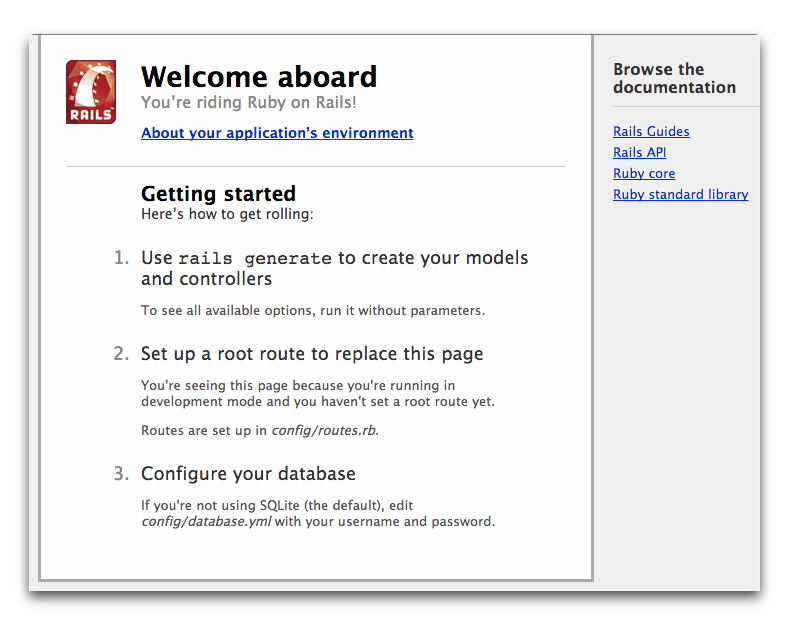
\includegraphics[width=12cm]{./image/rails/rails_welcome.png}
	\end{center}
\end{figure}

La página de ``Welcome aboard'' es un test para una nueva aplicación de \textit{Rails}. Con ello se asegura que \textit{Ruby on Rails} ha sido configurado de forma correcta. También se puede acceder al link ``About your application's environment'' para ver un resumen del entorno de la aplicación.

Para detener el servidor web, hay que presionar las teclas Ctrl+C en la ventana del terminal en la que el servidor web está siendo ejecutado.

\section{Modelos}
Como se ha dicho varias veces, \textit{Rails} usa el patrón de arquitectura MVC. Los modelos son la capa o parte del sistema responsable de representar la lógica de negocio. Los modelos de \textit{Rails} son diseñados y representados mediante Active Record.

\subsection{Active Record}
Active Record facilita la creación y uso de los objetos negocio cuyos datos precisan de ser persistentes en la base de datos.

Active Record es un objeto que envuelve una fila de una tabla o vista de una base de datos, encapsula el acceso a la base de datos, y añade lógica de negocio en esos datos envueltos. Active Record conlleva tanto tantos como comportamiento y muchos de estos datos deben de ser persistentes en la base de datos. Active Record añade acceso lógico a los datos en el dominio del objeto, de esta manera, todo el mundo sabe como leer y escribir los datos en la base de datos. \cite{Fowler2002}

Active Record es una descripción de ORM (Object-Relational-Mapping), que es una tecnica que conecta objetos de la aplicación con las tables de una base de datos relacional. Usando ORM, las propiedades de las relaciones de los objetos en una aplicación pueden ser facilmente almacenados y recuperados desde la base de datos, sin escribir consultas SQL directamente.

Active Record proporciona varios mecanismos propios de una técnica ORM:

\begin{enumerate}
	\item Representar modelos y sus datos.
	\item Representar asociaciones entre los modelos.
	\item Representar jerarquías de herencia a través de los modelos relacionados.
	\item Validar modelos antes de ser escritos de forma persistente a la base de datos.
	\item Realizar operaciones en la base de datos con una sintaxis y un estilo de orientación a objetos.
\end{enumerate}

\subsection{Convención sobre configuración en Active Record}
A diferencia de otros lenguajes de programación o frameworks, en \textit{Rails} no es necesario escribir mucha configuración cuando se trabaja con modelos de Active Record.

Por defecto, Active Record utiliza convenciones en los nombres para entender como un modelo y la la tabla de la base de datos deberían ser creados. \textit{Rails} pluraliza los nombres de las clases para encontrar la respectiva tabla de la base de datos. \footnote{La pluralización de \textit{Rails} es muy potente, siendo capaz de pluralizar o singularizar palabras regulares e irregulares.}

Active Record también utiliza convenciones para los nombres de las columnas de la base de datos, dependiendo del propósito de las columnas. 

\begin{description}
	\item[Claves ajenas] Los campos deben ser llamamos siguiendo el patrón nombre de la tabla singularizado e id. Por ejemplo, \texttt{user\_id} de la tabla \texttt{users}.
	\item[Claves primarias] Por defecto, Active Record utilizará una columna de tipo en tero llamada \texttt{id} como clave primaria.
\end{description}

\subsection{Creando modelos Active Record}

Para crear modelos de Active Record, lo único que se precisa hacer es asignarlo como subclase de \texttt{ActiveRecord::Base}

\begin{lstlisting}[language=Ruby]
class Product < ActiveRecord::Base
end
\end{lstlisting}

Esto permite crear un modelo \texttt{Product} que será referenciado a la tabla \texttt{products} de la base de datos. De esta manera, se posibilita la forma de referenciar columnas de cada fila de la tabla de la base de datos con los atributos de las instancias del modelo.


Suponiendo que la tabla productos ha sido creada utilizando la siguiente sentencia SQL,

\begin{lstlisting}[language=SQL]
CREATE TABLE products (
   id int(11) NOT NULL auto_increment,
   name varchar(255),
   PRIMARY KEY  (id)
);
\end{lstlisting}

Será posible escribir código como el siguiente:

\begin{lstlisting}[language=Ruby]
p = Product.new
p.name = "El Quijote"
puts p.name # "El Quijote"
\end{lstlisting}

\subsection{CRUD}
En computación CRUD es el acronimo de los cuatro verbos que usamos para operar con datos: Create, Read, Update y Delete. Active Record automaticamente crea estos métodos para permitir a la aplicación leer y manipular los datos almacenados en sus tablas.

\subsubsection{Create}
Los objetos de Active Record pueden ser creados desde un hash o manualmente establecidos después de su creación. El método \texttt{new} devuelve un objeto nuevo mientras que \texttt{create} retornará el objeto y lo almacenará en la base de datos.

El siguiente fragmento de código utiliza el método \texttt{create} por lo que creará el usuario y lo guardará como un nuevo registro en la base de datos.
\begin{lstlisting}[language=Ruby]
user = User.create(name: "Antonio", occupation: "Profesor")
\end{lstlisting}

Por el contrario, en este otro fragmento de código el usuario es creado pero no es guardado en la base de datos. 
\begin{lstlisting}[language=Ruby]
user = User.new
user.name = "Antonio"
user.occupation = "Profesor"
\end{lstlisting}

Si además se deseara guardar el usuario, se deberá utilizar el método \texttt{user.save}.

\subsubsection{Read}
Active Record proporciona una API potente para acceder a datos de la base de datos. A continuación se exponen una serie de ejemplos que ilustran los diferentes métodos facilitados por Active Record.


\begin{lstlisting}[language=Ruby]
# Devuelve una colección con todos los usuarios. 
users = User.all
\end{lstlisting}
 
\begin{lstlisting}[language=Ruby]
# Devuelve el primer usuario.
user = User.first 
\end{lstlisting}
 
\begin{lstlisting}[language=Ruby]
# Retorna el primer usuario con nombre Antonio
david = User.find_by(name: 'Antonio')  
\end{lstlisting}
  
\begin{lstlisting}[language=Ruby]
#Encuentra todos los usuarios llamados Antonio que son profesores ordenados por fecha de creación de forma inversa.
users = User.where(name: 'Antonio', occupation: 'Profesor').order(created_at: :desc)   
\end{lstlisting}

\subsubsection{Update}
Una vez que un objeto de Active Record ha sido recuperado, sus atributos pueden ser modificados y pueden ser guardados en la base de datos.

\begin{lstlisting}[language=Ruby]
user = User.find_by(name: 'David')
user.name = 'Antonio'
user.save
\end{lstlisting}

\begin{lstlisting}[language=Ruby]
# Otra forma de realizarlo
user = User.find_by(name: 'David')
user.update(name: 'Antonio')
\end{lstlisting}

\subsubsection{Delete}
Análogamente, un objeto de Active Record recuperado puede ser destruido, lo que le borra de la base de datos.

\begin{lstlisting}[language=Ruby]
user = User.find_by(name: 'Antonio')
user.destroy
\end{lstlisting}


\subsection{Migraciones de la base de datos}
Las migraciones de \textit{Rails} son la forma mas conveniente de alterar el esquema de la base de datos de una manera consistente y sencilla. Las migraciones usan un Ruby DSL (Domain Specific Language) por lo que no hace falta escribir ni una sola instrucción SQL, permitiendo que el esquema de la base de datos y los cambios ser independientes de la base de datos.

Se puede pensar que una migración es una nueva ``versión'' de la base de datos. Active Record actualiza el archivo \texttt{db/schema.rb} para mantener la estructura actualizada de la base de datos.

Un ejemplo de una migración:

\begin{lstlisting}[language=Ruby]
class CreateProducts < ActiveRecord::Migration
  def change
    create_table :products do |t|
      t.string :name
      t.text :description
 
      t.timestamps null: false
    end
  end
end
\end{lstlisting}

Las migraciones pueden ser lanzadas hacia ``delante'' o hacia ``detrás'', esto significa que si, por ejemplo, la migración anterior es lanzada cuando no existe la tabla \texttt{products} en la base de datos, entonces, la tabla \texttt{products} con las columnas \texttt{name}, \texttt{descripción}, y \texttt{timestamps} será creada. Por el contrario, si lanzamos la migración cuando la tabla existe en la base de datos, lo que se producirá es un efecto de \textit{rollback}.

En las bases de datos que soportan transacciones con instrucciones que modifiquen el esquema, las migraciones son envueltas en una transacción, de forma que si una migración falla, se hará un \textit{rollback} automáticamente de la transacción.\footnote{Si la base de datos no soporta transacciones y la migración falla, los cambios para hacer el rollback deben ser realizados manualmente.}

Algunas migraciones contienen ciertas instrucciones que Active Record no sabe como hacer el inverso de dicha operación. El ejemplo más típico es el cambio de nombre.

\begin{lstlisting}[language=Ruby]
class ChangeProductsPrice < ActiveRecord::Migration
  def up
    change_table :products do |t|
      t.change :price, :string
    end
  end
 
  def down
    change_table :products do |t|
      t.change :price, :integer
    end
  end
end
\end{lstlisting}


\subsubsection{Creando una migración simple}
Las migraciones son almacenadas en ficheros en el directorio \texttt{db/migrate}, un fichero por cada migración. El nombre del fichero contiene el UTC timestamp que es la fecha en formato YYYYMMDDHHMMSS (año, mes, día, hora, minuto, segundo) seguido de guión bajo y el nombre de la migración. \textit{Rails} usa el UTC timestamp para determinar el orden en el que las migraciones deben ser ejecutadas.

Se puede generar una migración de la siguiente forma:

\begin{lstlisting}[language=bash]
$ bin/rails generate migration AddPartNumberToProducts
\end{lstlisting}

Ese comando creará un nuevo archivo en \texttt{db/migrate} que contendrá:

\begin{lstlisting}[language=Ruby]
class AddPartNumberToProducts < ActiveRecord::Migration
  def change
  end
end
\end{lstlisting}

Si el nombre de la migración sigue el patrón AddXXXToYYY o RemoveXXXFromYYY seguido de una lista de nombres de columnas y sus tipos, entonces la migración será creada con las instrucciones \texttt{add\_column} y \texttt{remove\_column}, respectivamente.

\begin{lstlisting}[language=bash]
$ bin/rails generate migration AddPartNumberToProducts part_number:string
\end{lstlisting}

\begin{lstlisting}[language=Ruby]
lass AddPartNumberToProducts < ActiveRecord::Migration
  def change
    add_column :products, :part\_number, :string
  end
end
\end{lstlisting}


\myparagraph{Generadores de Modelos}
El modelo y los \textit{scaffold generators} crean las migraciones apropiadas para el nuevo modelo. Esta migración contendrá instrucciones para crear la tabla de la base de datos. 

\begin{lstlisting}[language=bash]
$ bin/rails generate model Product name:string description:text 
\end{lstlisting}  

El generador anterior creará el nuevo modelo y una migración nueva con el siguiente contenido:

\begin{lstlisting}[language=Ruby]
class CreateProducts < ActiveRecord::Migration
  def change
    create_table :products do |t|
      t.string :name
      t.text :description
 
      t.timestamps null: false
    end
  end
end
\end{lstlisting}


\subsubsection{Sintaxis de las migraciones}

\myparagraph{Tablas}
El método \texttt{create\_table} es el más fundamental y casi siempre es creado por un generador de modelos o un \textit{scaffold generator}. Implícitamente crea una columna \texttt{id} que será la clave primaria.

\begin{lstlisting}[language=Ruby]
create_table :products do |t|
  t.string :name
end
\end{lstlisting}

\myparagraph{Join Table}
El método de migración \texttt{create\_join\_table} crea una tabla join para una relación de muchos a muchos o HABTM.\footnote{Has and belongs to many}

\begin{lstlisting}[language=Ruby]
create_join_table :products, :categories
\end{lstlisting}

\begin{lstlisting}[language=Ruby]
create_join_table :products, :categories do |t|
  t.index :product_id
  t.index :category_id
end
\end{lstlisting}


\myparagraph{Modificación de columnas}
Los métodos de modificación de columnas son los siguientes:

\begin{lstlisting}[language=Ruby]
change_column :products, :part_number, :text
\end{lstlisting}

\begin{lstlisting}[language=Ruby]
add_column :products, :description, :string
\end{lstlisting}

\begin{lstlisting}[language=Ruby]
remove_column :products, :description
\end{lstlisting}

\subparagraph{Modificadores de columnas}
Los modificadores de columnas pueden aplicados cuando se crea o se modifica una columna.

\begin{description}
	\item[\texttt{limit}] Establece el tamaño máximo de los campos de tipo \texttt{string / text / binary / integer}
	\item[\texttt{precision}] Define la precisión para los campos de tipo \texttt{decimal}, representando el numero total de dígitos en el número.
	\item[\texttt{scale}] Define la escala para los campos de tipo \texttt{decimal}, representando el número de dígitos después del punto decimal. 
	\item[\texttt{polymorphic}] Este parámentro añade una columna del tipo \texttt{type} para las asociaciones \texttt{belongs\_to}.
	\item[\texttt{null}] Habilita o inhabilita valores de tipo \texttt{NULL} en la columna.
	\item[\texttt{default}] Permite establecer un valor por defecto en la columna.
	\item[\texttt{index}] Añade un índice a la columna.
	\item[\texttt{required}] Añade \texttt{required: true} para las asociaciones \texttt{belongs\_to} y \texttt{null: false} a la columna en la migración.
\end{description}

\myparagraph{Claves ajenas}
Las claves ajenas ayudan a mantener la integridad referencial de una base de datos.

\begin{lstlisting}[language=Ruby]
add_foreign_key :articles, :authors
\end{lstlisting}

Añade la clave ajena, introduciendo la columna \texttt{author\_id} en la tabla \texttt{articles}. La clave referencia a la columna \texttt{id} en la tabla \texttt{authors}.

Active Record solo soporta claves ajenas de una sola columna. Para claves ajenas compuestas se precisa \texttt{execute} y \texttt{structure.sql}.

Hay varias opciones para eliminar claves ajenas:

\begin{lstlisting}[language=Ruby]
# Active Record buscará el nombre de columna.
remove_foreign_key :accounts, :branches

#Elimina la clave ajena de una columna especifica.
remove_foreign_key :accounts, column: :owner_id
 
# Elimina la clave ajena por su nombre.
remove_foreign_key :accounts, name: :special_fk_name
\end{lstlisting}

\myparagraph{Ejecutar SQL}
Si Active Record no fuera suficiente, se pueden ejecutar instrucciones directamente en lenguaje SQL mediante el método \texttt{execute}.\footnote{Documentación relacionada en la API de \textit{Ruby on Rails}, \url{http://api.rubyonrails.org/classes/ActiveRecord/ConnectionAdapters/SchemaStatements.html}}

\begin{lstlisting}[language=Ruby]
Product.connection.execute('UPDATE `products` SET `price`=`free` WHERE 1')
\end{lstlisting}

\myparagraph{Rollback}
Como se ha mencionado anteriormente, \textit{Rails} soporta rollbacks de las migraciones a la base de datos, porporcionando diversos métodos:

\subparagraph{Método \texttt{change}}
El método \texttt{change} es el método primario y por defecto de las migraciones. Funciona en la mayoría de los casos que son aquellos en los cuales Active Record sabe cual es la migración inversa. El método \texttt{change} soporta las siguientes definiciones:

\begin{enumerate}
	\item add\_column
	\item add\_index
	\item add\_reference
	\item add\_timestamps
	\item add\_foreign\_key
	\item add\_table
	\item add\_join\_table
	\item drop\_table (si se proporciona un bloque con el contenido)
	\item drop\_join\_table (si se proporciona un bloque con el contenido)
	\item remove\_timestamps
	\item rename\_column
	\item rename\_index
	\item rename\_reference
	\item rename\_table
\end{enumerate}

\subparagraph{Método \texttt{reversible}}
Otros métodos o algunas migraciones complejas requieren procesado que Active Record no sabe como hacer la operación inversa. Para solucionarlo, el método \texttt{reversible} permite especificar que se debe de hacer cuando se ejecuta una migración y cuando se revierte una migración.

\begin{lstlisting}[language=Ruby]
class ExampleMigration < ActiveRecord::Migration
  def change
    create_table :distributors do |t|
      t.string :zipcode
    end
 
    reversible do |dir|
      dir.up do
        # add a CHECK constraint
        execute <<-SQL
          ALTER TABLE distributors
            ADD CONSTRAINT zipchk
              CHECK (char_length(zipcode) = 5) NO INHERIT;
        SQL
      end
      dir.down do
        execute <<-SQL
          ALTER TABLE distributors
            DROP CONSTRAINT zipchk
        SQL
      end
    end
 
    add_column :users, :home_page_url, :string
    rename_column :users, :email, :email_address
  end
end
\end{lstlisting}

En lo casos en los que una migración sea totalmente irreversible, como cuando se destruyen algunos datos, se puede lanzar una excepción de \texttt{ActiveRecord::IrreversibleMigration} en el bloque \texttt{down}, de forma que si alguien intenta realizar la migración, un mensaje de error será emitido.

\subparagraph{Método \texttt{up/down}}

Además de el método reversible, existe el método \texttt{up/down} que similar funcionalmente pero la sintaxis es distinta.

\begin{lstlisting}[language=Ruby]
class ExampleMigration < ActiveRecord::Migration
  def up
    create_table :distributors do |t|
      t.string :zipcode
    end
 
    # add a CHECK constraint
    execute <<-SQL
      ALTER TABLE distributors
        ADD CONSTRAINT zipchk
        CHECK (char_length(zipcode) = 5);
    SQL
 
    add_column :users, :home_page_url, :string
    rename_column :users, :email, :email_address
  end
 
  def down
    rename_column :users, :email_address, :email
    remove_column :users, :home_page_url
 
    execute <<-SQL
      ALTER TABLE distributors
        DROP CONSTRAINT zipchk
    SQL
 
    drop_table :distributors
  end
end
\end{lstlisting}


\subsubsection{Ejecución de migraciones}
\textit{Rails} proporciona un conjunto de tareas Rake para ejecutar migraciones.
La migración sencilla ejecuta el método \texttt{change} o el método \texttt{up} para todas las migraciones que aún no han sido ejecutadas. Si no hay migraciones, estas se ejecutarán en base al orden de creación de su UTC timestamp. 

\begin{lstlisting}[language=bash]
$ bin/rake db:migrate
\end{lstlisting}

Si se especifica una versión, Active Record ejecutará las migraciones requeridas (\texttt{change}, \texttt{up}, \texttt{down}) hasta que se alcance la versión especificada.

\begin{lstlisting}[language=bash]
$ bin/rake db:migrate VERSION=20150906120000
\end{lstlisting}

\myparagraph{Rollback}
Un rollback habitual es volver a la migración anterior debido a un error, por ejemplo.

\begin{lstlisting}[language=bash]
$ bin/rake db:rollback
\end{lstlisting}

Mediante el parámetro \texttt{STEP}, especificamos cuantas migraciones se deben revertir.

\begin{lstlisting}[language=bash]
$ bin/rake db:rollback STEP=3
\end{lstlisting}

Si se desea revertir una o varias migraciones y luego migrar otra vez, existe un atajo:

\begin{lstlisting}[language=bash]
$ bin/rake db:migrate:redo STEP=3
\end{lstlisting}

Por último, y como consecuencia lógica de la funcionalidad cuando se especifica una version concreta, si se pretende revertir hasta cierto punto o momento, se debe especificar con el parámetro \texttt{VERSION}.

\begin{lstlisting}[language=bash]
$ bin/rake db:migrate VERSION=20150906120000
\end{lstlisting}

\myparagraph{Otras tareas Rake}
Otras tareas y operaciones con Rake frecuentes son las siguientes:

\begin{description}
	\item[\texttt{rake db:setup}] Esta tarea crea la base de datos, carga el esquema y la inicializa con los datos semilla.
	\item[\texttt{rake db:drop}] Esta operación destruye la base de datos y el esquema.
	\item[\texttt{rake db:reset}] Esta operación es similar a realizar \texttt{rake db:drop} y después \texttt{rake db:setup}.\footnote{Esta operación no es lo mismo que ejecutar todas las migraciones. Sólo usará los contenidos del archivo \texttt{schema.rb} actual. Si una migración no puede ser revertida, \texttt{rake db:reset} no será útil probablemente.} 
\end{description}

Por defecto, \texttt{rake db:migrate} es una instrucción que siempre se ejecutará en modo desarrollo (\texttt{development}). Si se desea ejecutar migraciones en otro entorno que no sea el de desarrollo se puede especificar usando la variable \texttt{RAILS\_ENV} mientras se ejecuta el comando.

\begin{lstlisting}[language=bash]
$ bin/rake db:migrate RAILS_ENV=test
\end{lstlisting}

\begin{lstlisting}[language=bash]
$ bin/rake db:rollback RAILS_ENV=production
\end{lstlisting}

\myparagraph{Migraciones y datos semilla}
Se pueden usar migraciones para añadir datos a la base de datos:

\begin{lstlisting}[language=Ruby]
class AddInitialProducts < ActiveRecord::Migration
  def up
    5.times do |i|
      Product.create(name: "Product ##{i}", description: "A product.")
    end
  end
 
  def down
    Product.delete_all
  end
end
\end{lstlisting}

Sin embargo, \textit{Rails} tiene una funcionalidad de semillas que será usada para poblar bases de datos. Se trata añadir código al archivo \texttt{db/seeds.rb} y después, ejecuta el comando \texttt{rake db:seed}.

\begin{lstlisting}[language=Ruby]
5.times do |i|
  Product.create(name: "Product ##{i}", description: "A product.")
end
\end{lstlisting} 


\subsection{Validaciones}
\subsubsection{Introducción}

Validación es el proceso que garantiza que un dato o conjunto de datos cumple con los requisitos y especificaciones necesarias para ser introducido en el sistema de forma persistente.

\begin{lstlisting}[language=Ruby]
class Person < ActiveRecord::Base
  validates :name, presence: true
end
 
Person.create(name: "Thomas A. Anderson").valid? # => true
Person.create(name: nil).valid? # => false
\end{lstlisting}
 
Las validaciones a nivel de modelo son la mejor forma en \textit{Rails} para asegurar que los datos datos que se guardan en la base de datos son correctos.
Además de validar los datos a nivel de modelo, existen otras formas de validar los datos:

\begin{enumerate}
	\item Restricciones y procedimientos almacenados que hacen la validación dependiente de la base de datos por lo que el testeo y el mantenimiento es más complicado. Sin embargo, si la base de datos es utilizada por otras aplicaciones, es ventajoso poner las restricciones a nivel de la base de datos.
	\item Las validaciones en el cliente pueden ser útiles pero no fiables si se usan por si mismas.
	\item Las validaciones al nivel del controlador son difíciles de testear y mantener. Siguiendo una de las filosofias de \textit{Ruby on Rails}, lso controladores deben ser simples en cuanto a complejidad mientras que los modelos deben complejos.
\end{enumerate}

Hay muchas formas de cambiar los estados de los objetos en la base de datos. Algunos métodos implican la ejecución de disparadores de validación, pero otros no. Por tanto, es posible guardar un objeto inválido en la base de datos si no se trata con cuidado.

Los siguientes métodos lanzan validaciones. La diferencia es que los que tienen exclamación lanzan una excepción si el objeto es inválido mientras que los otros retornan false (\texttt{save} y \texttt{update}) o el objeto (\texttt{create}).
 
\begin{enumerate}
	\item \texttt{create}
	\item \texttt{create!}
	\item \texttt{save}
	\item \texttt{save!}
	\item \texttt{update}
	\item \texttt{update!}
\end{enumerate}

Los siguientes métodos saltan las validaciones, y por tanto, guardarán el objeto en la base de dato independientemente de su validez:

\begin{enumerate}
	\item \texttt{decrement!}
	\item \texttt{decrement\_counter}
	\item \texttt{increment!}
	\item \texttt{increment\_counter}
	\item \texttt{toggle!}
	\item \texttt{update\_all}
	\item \texttt{update\_attribute}
	\item \texttt{update\_column}
	\item \texttt{update\_columns}
	\item \texttt{update\_counters}
	\item Además \texttt{save} también tiene la habilidad de saltar validaciones si utiliza con el argumento \texttt{validate: false}.
\end{enumerate}

Para verificar si un objeto es válido o inválido, \textit{Rails} usa el método \texttt{valid?}.

\begin{lstlisting}[language=Ruby]
class Person < ActiveRecord::Base
  validates :name, presence: true
end
 
Person.create(name: "Thomas A. Anderson").valid? # => true
Person.create(name: nil).valid? # => false
\end{lstlisting}

Un objeto instanciado con el método \texttt{new} no reportará errores de validación incluso si es inválido debido a que las validaciones no son disparadas cuando se utiliza el método \texttt{new}.

\begin{lstlisting}[language=Ruby]
class Person < ActiveRecord::Base
  validates :name, presence: true
end
 
>> p = Person.new
# => #<Person id: nil, name: nil>
>> p.errors.messages
# => {}
 
>> p.valid?
# => false
>> p.errors.messages
# => {name:["can't be blank"]}
 
>> p = Person.create
# => #<Person id: nil, name: nil>
>> p.errors.messages
# => {name:["can't be blank"]}
 
>> p.save
# => false
 
>> p.save!
# => ActiveRecord::RecordInvalid: Validation failed: Name can't be blank
 
>> Person.create!
# => ActiveRecord::RecordInvalid: Validation failed: Name can't be blank
\end{lstlisting}

Para verificar si un atributo en particular de un objeto es válido, se puede utilizar el método \texttt{errors[:attribute]}. El método retorna un vector con todos los errores del atributo \texttt{:attribute}. Si no hay errores en dicho atributo, un array vació será retornado.

\begin{lstlisting}[language=Ruby]
class Person < ActiveRecord::Base
  validates :name, presence: true
end
 
>> Person.new.errors[:name].any? # => false
>> Person.create.errors[:name].any? # => true
\end{lstlisting}


\subsubsection{Procedimientos de validación}

Active Record proporciona un conjunto de procedimientos de validación que pueden ser directamente usados en las clases. Estos procedimientos proporcionan reglas comunes de validación. Siempre que una validación falla, un mensaje de error es añadido a la colección de errores del objeto con un mensaje asociado al atributo validado.

\myparagraph{\texttt{acceptance}}
Éste método valida que una checkbox en el interfaz de usuario ha sido seleccionada cuando el formulario ha sido enviado. El mensaje de error por defecto es ``must be accepted''.

\begin{lstlisting}[language=Ruby]
class Person < ActiveRecord::Base
  validates :terms_of_service, acceptance: true
end
\end{lstlisting}

\myparagraph{\texttt{validates\_associated}}
El método \texttt{validates\_associated} debe ser utilizado cuando el modelo tiene asociaciones con otros modelos que también necesitan ser validados.\footnote{Es importante no utilizar el método \texttt{validates\_associated} en ambos extremos de la asociación, puesto que se llamarán unos a otros creando un bucle infinito.} El mensaje de error por defecto del método es ``is invalid''.

\begin{lstlisting}[language=Ruby]
class Library < ActiveRecord::Base
  has_many :books
  validates_associated :books
end
\end{lstlisting}

\myparagraph{\texttt{confirmation}}
Éste procedimiento se puede utilizar cuando dos campos de texto reciben exactamente el mismo contenido como en una validación de una contraseña. El mensaje de error por defecto es ``doesn't match confirmation''.

\begin{lstlisting}[language=Ruby]
#Modelo
class Person < ActiveRecord::Base
  validates :email, confirmation: true
end 

#Vista
<%= text_field :person, :email %>
<%= text_field :person, :email_confirmation %>
\end{lstlisting}


\myparagraph{\texttt{exclusion}}
El procedimiento \texttt{exclusion} valida que los valores de los atributos no estén incluidos en un conjunto dado. Éste método, además, incorpora una opción \texttt{:in} que recibe un conjunto de valores que no serán aceptados por el atributo al ser validado.\footnote{La opción \texttt{:in} posee un alias \texttt{:within} que realiza la misma funcionalidad.} El mensaje de error es ìs reserved''.

\begin{lstlisting}[language=Ruby]
class Account < ActiveRecord::Base
  validates :subdomain, exclusion: { in: %w(www us ca jp),
    message: "%{value} is reserved." }
end
\end{lstlisting}

\myparagraph{\texttt{format}}
El método \texttt{format} valida los valores de los atributos probando si coinciden o no con una expresión regular dada con la opción \texttt{:with} o \texttt{:without}, respectivamente. Por defecto, su mensaje de error es ``is invalid''.

\begin{lstlisting}[language=Ruby]
class Product < ActiveRecord::Base
  validates :legacy_code, format: { with: /\A[a-zA-Z]+\z/,
    message: "only allows letters" }
end
\end{lstlisting}

\myparagraph{\texttt{inclusion}}
Éste procedimiento es inverso al método \texttt{exclusion} y por tanto, valida que los valores de los atributos son incluidos en un conjunto dado. De la misma manera que \texttt{exclusion}, éste método posee las opciones \texttt{:in} o \texttt{:within}.

\begin{lstlisting}[language=Ruby]
class Coffee < ActiveRecord::Base
  validates :size, inclusion: { in: %w(small medium large),
    message: "%{value} is not a valid size" }
end
\end{lstlisting}

\myparagraph{\texttt{length}}
El método \texttt{length} valida que los valores de los atributos tengan una longitud concreta. Provee una serie de opciones, por lo que se puede especificar constantes de longitud de diversas formas.

\begin{description}
	\item[\texttt{:minumum}] El atributo no puede ser menor que la longitud especificada.
	\item[\texttt{:maximum}] El atributo no puede ser mayor que la longitud especificada.
	\item[\texttt{:in} o \texttt{:within}] El atributo debe estar incluido en el rango de la longitud especificada.
	\item[\texttt{:is}] El atributo deber ser igual que la longitud especificada.
\end{description}

\begin{lstlisting}[language=Ruby]
class Essay < ActiveRecord::Base
  validates :content, length: {
    minimum: 300,
    maximum: 400,
    tokenizer: lambda { |str| str.split(/\s+/) },
    too_short: "must have at least %{count} words",
    too_long: "must have at most %{count} words"
  }
end
\end{lstlisting}


\myparagraph{\texttt{numericality}}
El procedimiento valida que los atributos solo contengan valores numéricos. Por defecto, acepta cualquier valor numérico pero puede ser restringido a sólo enteros o flotantes. El error por defecto es ``is not a number''.

\begin{description}
	\item[\texttt{:greater\_than}] Especifica que el valor deber ser mayor que el valor proporcionado.
	\item[\texttt{:greater\_than\_or\_equal\_to}] Especifica que el valor deber ser mayor o igual que el valor proporcionado.
	\item[\texttt{:equal\_to}] Especifica que el valor deber ser igual que el valor proporcionado.
	\item[\texttt{:less\_than}] Especifica que el valor deber ser menor que el valor proporcionado.
	\item[\texttt{:less\_than\_or\_equal\_to}] Especifica que el valor deber ser menor o igual que el valor proporcionado.
	\item[\texttt{:odd}] Especifica que el valor debe ser impar.
	\item[\texttt{:even}] Especifica que el valor debe ser par.
\end{description} 

\myparagraph{\texttt{presence}}
Éste método valida que los atributos especificados con él no son vacíos.

\begin{lstlisting}[language=Ruby]
class Person < ActiveRecord::Base
  validates :name, :login, :email, presence: true
end
\end{lstlisting}

También puede ser utilizado para asegurar que una asociación es presente.

\begin{lstlisting}[language=Ruby]
class LineItem < ActiveRecord::Base
  belongs_to :order
  validates :order, presence: true
end

class Order < ActiveRecord::Base
  has_many :line_items, inverse_of: :order
end
\end{lstlisting}

\myparagraph{\texttt{absence}}
De forma contraria al método \texttt{presence}, éste procedimiento asegura los atributos especificados no son presentes.

\begin{lstlisting}[language=Ruby]
class Person < ActiveRecord::Base
  validates :name, :login, :email, absence: true
end
\end{lstlisting}

Analogamente al procedimiento \texttt{presence}, también puede ser utilizado para asegurar asociaciones.

\begin{lstlisting}[language=Ruby]
class LineItem < ActiveRecord::Base
  belongs_to :order
  validates :order, absence: true
end

class Order < ActiveRecord::Base
  has_many :line_items, inverse_of: :order
end
\end{lstlisting}

\myparagraph{\texttt{uniqueness}}
El procedimiento \texttt{uniqueness} valida que los valores de atributo son únicos antes de que el objeto sea guardado en la base de datos. El mensaje de error por defecto es ``has already been taken''. 

\begin{lstlisting}[language=Ruby]
class Account < ActiveRecord::Base
  validates :email, uniqueness: true
end
\end{lstlisting}

La opción \texttt{:scope} permite especificar otros atributos que son utilizados para limitar la validación

\begin{lstlisting}[language=Ruby]
class Holiday < ActiveRecord::Base
  validates :name, uniqueness: { scope: :year,
    message: "should happen once per year" }
end
\end{lstlisting}

La opción \texttt{:case\_sensitive} define si la unicidad debe ignorar mayúsculas y minúsculas.

\myparagraph{\texttt{validates\_with}}
Éste método pasa el registro a otra clase para emprender la validación.

\begin{lstlisting}[language=Ruby]
class GoodnessValidator < ActiveModel::Validator
  def validate(record)
    if record.first_name == "Evil"
      record.errors[:base] << "This person is evil"
    end
  end
end
 
class Person < ActiveRecord::Base
  validates_with GoodnessValidator
end
\end{lstlisting}


\subsubsection{Opciones de validación}

Las opciones de validación más comunes son:

\begin{description}
	\item[\texttt{:allow\_nil}] Salta la validación cuando el valor evaluado es \texttt{nil}.
\begin{lstlisting}[language=Ruby]
  class Coffee < ActiveRecord::Base
    validates :size, inclusion: { in: %w(small medium large),
      message: "%{value} is not a valid size" }, allow_nil: true
  end
\end{lstlisting}

	\item[\texttt{:allow\_blank}] Ésta opción ignora la validación si el valor es \texttt{nil} o una cadena de texto vacía.	
\begin{lstlisting}[language=Ruby]
class Topic < ActiveRecord::Base
  validates :title, length: { is: 5 }, allow_blank: true
end
 
Topic.create(title: "").valid?  # => true
Topic.create(title: nil).valid? # => true
\end{lstlisting}

	\item[\texttt{:message}] La opción \texttt{:message} permite especificar el mensaje que será añadido a la colección de errores cuando la validación falla.
	
	\item[\texttt{:on}] Permite especificar cuando la validación debe ocurrir.
	
\begin{lstlisting}[language=Ruby]
class Person < ActiveRecord::Base
  # it will be possible to update email with a duplicated value
  validates :email, uniqueness: true, on: :create
 
  # it will be possible to create the record with a non-numerical age
  validates :age, numericality: true, on: :update
 
  # the default (validates on both create and update)
  validates :name, presence: true
end	
\end{lstlisting}
	
\end{description}

\subsubsection{Validación condicional}
Se puede validar un objeto solamente cuando cierta condición es satisfecha. Para ello, \textit{Rails} habilita los métodos \texttt{:if} y \texttt{unless}.

\begin{description}
	\item[\texttt{Symbol} con \texttt{:if} y \texttt{:unless}] Se puede asociar \texttt{:if} y \texttt{:unless} con un símbolo que corresponde con el nombre un método que será llamado cuando la validación ocurre.

\begin{lstlisting}[language=Ruby]
class Order < ActiveRecord::Base
  validates :card_number, presence: true, if: :paid_with_card?
 
  def paid_with_card?
    payment_type == "card"
  end
end
\end{lstlisting}

	\item[Cadena de caracteres con \texttt{:if} y \texttt{:unless}] Es posible utilizar una cadena que será evaluada con el método \texttt{eval}. 

\begin{lstlisting}[language=Ruby]
class Person < ActiveRecord::Base
  validates :surname, presence: true, if: "name.nil?"
end
\end{lstlisting}

	\item[Proc con \texttt{:if} y \texttt{:unless}] También es posible asociar \texttt{:if} y \texttt{:unless} con un objeto de la clase \texttt{Proc} que se será llamado. 

\begin{lstlisting}[language=Ruby]
class Account < ActiveRecord::Base
  validates :password, confirmation: true,
    unless: Proc.new { |a| a.password.blank? }
end
\end{lstlisting}

\end{description}

\myparagraph{Agrupado y combinado de validaciones}
Resulta útil y clarificador poder combinar múltiples condiciones en una sola condición.

\begin{lstlisting}[language=Ruby]
class User < ActiveRecord::Base
  with_options if: :is_admin? do |admin|
    admin.validates :password, length: { minimum: 10 }
    admin.validates :email, presence: true
  end
end
\end{lstlisting}

De la misma manera se pueden combinar condiciones múltiples cuando una validación debe ocurrir o no.

\begin{lstlisting}[language=Ruby]
class Computer < ActiveRecord::Base
  validates :mouse, presence: true,
                    if: ["market.retail?", :desktop?],
                    unless: Proc.new { |c| c.trackpad.present? }
end
\end{lstlisting}

\subsubsection{Validaciones personalizadas}
Las validaciones personalizadas son creadas a través de clases que heredan de la clase \texttt{ActiveModel::Validator}. Éstas clases deben implementar un método \texttt{validate} que toma un argumento y le aplica la validación. Las validaciones personalizadas son ejecutadas llamando al método \texttt{validates\_with}.

\begin{lstlisting}[language=Ruby]
class MyValidator < ActiveModel::Validator
  def validate(record)
    unless record.name.starts_with? 'X'
      record.errors[:name] << 'Need a name starting with X please!'
    end
  end
end
 
class Person
  include ActiveModel::Validations
  validates_with MyValidator
end
\end{lstlisting}

También se pueden crear métodos personalizados que verifiquen el estado de los modelos y añadan mensajes a la colección de errores cuando son inválidos.

\begin{lstlisting}[language=Ruby]
class Invoice < ActiveRecord::Base
  validate :expiration_date_cannot_be_in_the_past,
    :discount_cannot_be_greater_than_total_value
 
  def expiration_date_cannot_be_in_the_past
    if expiration_date.present? && expiration_date < Date.today
      errors.add(:expiration_date, "can't be in the past")
    end
  end
 
  def discount_cannot_be_greater_than_total_value
    if discount > total_value
      errors.add(:discount, "can't be greater than total value")
    end
  end
end
\end{lstlisting}


\subsection{Callbacks}

Los \textit{callbacks} son métodos que son invocados en ciertos momentos de la vida de los objetos. Con ellos es posible escribir código que será ejecutado cuando un objeto Active Record es creado, guardado, actualizado, borrado, validado, o cargado de la base de datos.

\begin{lstlisting}[language=Ruby]
class User < ActiveRecord::Base
  validates :login, :email, presence: true
 
  before_validation :ensure_login_has_a_value
 
  protected
    def ensure_login_has_a_value
      if login.nil?
        self.login = email unless email.blank?
      end
    end
end
\end{lstlisting}



\myparagraph{Callbacks disponibles}
Los \textit{callbacks} de \textit{Rails} disponibles son los siguientes:

\begin{itemize}
	\item Creación del objeto
	\begin{itemize}
		\item \texttt{before\_validation}
		\item \texttt{after\_validation}
		\item \texttt{before\_save}
		\item \texttt{around\_save}
		\item \texttt{before\_create}
		\item \texttt{around\_create}
		\item \texttt{after\_create}
		\item \texttt{after\_save}
		\item \texttt{after\_commit} o \texttt{after\_rollback}
	\end{itemize}
	\item Actualización del objeto
	\begin{itemize}
		\item \texttt{before\_validation}
		\item \texttt{after\_validation}
		\item \texttt{before\_save}
		\item \texttt{around\_save}
		\item \texttt{before\_update}
		\item \texttt{around\_update}
		\item \texttt{after\_update}
		\item \texttt{after\_save}
		\item \texttt{after\_commit} o \texttt{after\_rollback} 
	\end{itemize}
	\item Destrucción del objeto
	\begin{itemize}
		\item \texttt{before\_destroy}
		\item \texttt{around\_destroy}
		\item \texttt{after\_destroy}
		\item \texttt{after\_commit} o \texttt{after\_rollback}
	\end{itemize}
	\item Otros \textit{callbacks}
	\begin{itemize}
		\item \texttt{after\_initialize} es un \textit{callback} que será invocado cuando el objeto de Active Record es instanciado, ya sea mediante el método \texttt{new} o cargado desde la base de datos.
		\item \texttt{after\_find} es un \textit{callback} llamado cuando un objeto Active Record es cargado desde la base de datos.
		\item \texttt{after\_touch} es un \textit{callback} invocado cada vez que un objeto de Active Record es tocado. 
	\end{itemize}		
\end{itemize}



\myparagraph{Ejecución de callbacks}
En \textit{Rails}, los métodos siguientes disparan \textit{callbacks}:

\begin{itemize}
	\item \texttt{create}
	\item \texttt{create!}
	\item \texttt{decrement!}
	\item \texttt{destroy}
	\item \texttt{destroy!}
	\item \texttt{destroy\_all}
	\item \texttt{increment!}
	\item \texttt{save}
	\item \texttt{save!}
	\item \texttt{save(validate: false)}
	\item \texttt{toggle!}
	\item \texttt{update\_attribute}
	\item \texttt{update}
	\item \texttt{update!}
	\item \texttt{valid?}
\end{itemize}

Adicionalmente, el \textit{callback} \texttt{after\_find} es disparado por los siguientes métodos de búsqueda.

\begin{itemize}
	\item \texttt{all}
	\item \texttt{first}
	\item \texttt{find}
	\item \texttt{find\_by}
	\item \texttt{find\_by\_*}
	\item \texttt{find\_by\_*!}
	\item \texttt{find\_by\_sql}
	\item \texttt{last}
\end{itemize}

\myparagraph{Callbacks relacionales}
Los \textit{callbacks} de \textit{Rails} pueden funcionar en relaciones de modelos, y pueden incluso ser definidas por las propias relaciones. Puede darse el caso de que cuando un objeto es destruido, también deberian ser destruidos los objetos que dependen del susodicho objeto.

\begin{lstlisting}[language=Ruby]
class User < ActiveRecord::Base
  has_many :articles, dependent: :destroy
end
 
class Article < ActiveRecord::Base
  after_destroy :log_destroy_action
 
  def log_destroy_action
    puts 'Article destroyed'
  end
end
 
>> user = User.first
=> #<User id: 1>
>> user.articles.create!
=> #<Article id: 1, user_id: 1>
>> user.destroy
Article destroyed
=> #<User id: 1>
\end{lstlisting}

\myparagraph{Callbacks condicionales}
De la misma forma que las validaciones, podemos ejecutar un \textit{callback} siempre y cuando se ejecute una condición concreta. Análogamente a las validaciones, los mecanismos empleados para los \textit{callbacks} condicionales son los mismos.

\begin{description}
	\item[\texttt{Symbol}] Las opciones \texttt{:if} y \texttt{:unless} pueden ser asociadas con un símbolo correspondiente al nombre de un método que será llamado antes de realizar el \textit{callback}.
\begin{lstlisting}[language=Ruby]
class Order < ActiveRecord::Base
  before_save :normalize_card_number, if: :paid_with_card?
end
\end{lstlisting}

	\item[Cadena de caracteres] Una cadena de caracteres de código \textit{Ruby} es admitida utilizando el método eval.
\begin{lstlisting}[language=Ruby]
class Order < ActiveRecord::Base
  before_save :normalize_card_number, if: "paid_with_card?"
end
\end{lstlisting}

	\item[\texttt{Proc}] \textit{Rails} posibilita la asociación a un objeto \texttt{Proc}.
\begin{lstlisting}[language=Ruby]
class Order < ActiveRecord::Base
  before_save :normalize_card_number,
    if: Proc.new { |order| order.paid_with_card? }
end
\end{lstlisting}

	\item[Callbacks con condiciones múltiples]
\begin{lstlisting}[language=Ruby]
class Comment < ActiveRecord::Base
  after_create :send_email_to_author, if: :author_wants_emails?,
    unless: Proc.new { |comment| comment.article.ignore_comments? }
end
\end{lstlisting}
\end{description}

\myparagraph{Clases callback}
\textit{Rails} permite crear clases que encapsulan métodos \textit{callback}, lo que facilita que otros modelos reutilicen esos \textit{callbacks}.

\begin{lstlisting}[language=Ruby]
class PictureFileCallbacks
  def after_destroy(picture_file)
    if File.exist?(picture_file.filepath)
      File.delete(picture_file.filepath)
    end
  end
end

class PictureFile < ActiveRecord::Base
  after_destroy PictureFileCallbacks.new
end
\end{lstlisting}


\subsection{Asociaciones de Active Record}

Las asociaciones facilitan y clarifican la manipulación y las operaciones sobre los objetos. Las asociaciones Active Record de \textit{Rails} permiten declarar a \textit{Rails} una conexión entre dos modelos especificando además de que tipo es.

\subsubsection{Tipos de asociaciones}
En \textit{Rails}, una asociación es una conexión entre dos modelos de Active Record. Las asociaciones son implementadas usando el estilo macro, por lo que es posible especificar y añadir características a los modelos.

\myparagraph{Asociación \texttt{belongs\_to}}
Ésta asociación establece una conexión de un modelo $\alpha$ de uno-a-muchos con otro modelo $\beta$. Para especificar el tipo de relación, la sintaxis\footnote{La asociación \texttt{belongs\_to} emplea el singular del modelo al especificado.} se realiza de la siguiente forma:

\begin{lstlisting}[language=Ruby]
class Order < ActiveRecord::Base
  belongs_to :customer
end
\end{lstlisting}


\includegraphics[width=10cm]{./image/logos/uahlogo3.png}

La migración será de la siguiente forma:

\begin{lstlisting}[language=Ruby]
class CreateOrders < ActiveRecord::Migration
  def change
    create_table :customers do |t|
      t.string :name
      t.timestamps null: false
    end
 
    create_table :orders do |t|
      t.belongs_to :customer, index: true
      t.datetime :order_date
      t.timestamps null: false
    end
  end
end
\end{lstlisting}


\myparagraph{Asociación \texttt{has\_one}}
La asociación \texttt{has\_one} es una conexión de uno-a-uno con otro modelo. Aunque parecida a la asociación anterior, ésta indica que cada instancia del modelo $\alpha$ contiene o posee una y sólo una instancia del modelo $\beta$. Para declarar dicha asociación, se procede de la siguiente forma:\footnote{Análogamente a la asociación \texttt{belongs\_to}, ésta también utiliza el singular del modelo al que se refiere.}

\begin{lstlisting}[language=Ruby]
class Supplier < ActiveRecord::Base
  has_one :account
end
\end{lstlisting}


\includegraphics[width=10cm]{./image/logos/uahlogo3.png}

La migración será de la siguiente forma:

\begin{lstlisting}[language=Ruby]
class CreateSuppliers < ActiveRecord::Migration
  def change
    create_table :suppliers do |t|
      t.string :name
      t.timestamps null: false
    end
 
    create_table :accounts do |t|
      t.belongs_to :supplier, index: true
      t.string :account_number
      t.timestamps null: false
    end
  end
end
\end{lstlisting}


\myparagraph{Asociación \texttt{has\_many}}
La asociación \texttt{has\_many} indica la relación de un modelo $\alpha$ de uno-a-muchos con otro modelo $\beta$. Es común encontrar esta asociación con la relación \texttt{belongs\_to} en el otro modelo. La asociación indica que instancia del modelo tiene cero o varias instancias del otro modelo.\footnote{Se escribir nombre del modelo en forma plural en la declaración de la relación. }

\begin{lstlisting}[language=Ruby]
class Customer < ActiveRecord::Base
  has_many :orders
end
\end{lstlisting}


\includegraphics[width=10cm]{./image/logos/uahlogo3.png}

La migración será de la siguiente forma:

\begin{lstlisting}[language=Ruby]
class CreateCustomers < ActiveRecord::Migration
  def change
    create_table :customers do |t|
      t.string :name
      t.timestamps null: false
    end
 
    create_table :orders do |t|
      t.belongs_to :customer, index:true
      t.datetime :order_date
      t.timestamps null: false
    end
  end
end
\end{lstlisting}


\myparagraph{Asociación \texttt{has\_many :through}}
Ésta asociación es usada frecuentemente cuando se pretende establecer una relación de muchos-a-muchos con otro modelo. La relación indica que el modelo $\alpha$ de la declaración puede tener cero o varias instancias del otro modelo $\beta$ a través (\texttt{:thrrough}) de un modelo $\gamma$ intermedio.

\begin{lstlisting}[language=Ruby]
class Doctor < ActiveRecord::Base
  has_many :appointments
  has_many :patients, through: :appointments
end
 
class Appointment < ActiveRecord::Base
  belongs_to :doctor
  belongs_to :patient
end
 
class Patient < ActiveRecord::Base
  has_many :appointments
  has_many :doctors, through: :appointments
end
\end{lstlisting}


\includegraphics[width=10cm]{./image/logos/uahlogo3.png}

La migración será de la siguiente forma:

\begin{lstlisting}[language=Ruby]
class CreateAppointments < ActiveRecord::Migration
  def change
    create_table :doctors do |t|
      t.string :name
      t.timestamps null: false
    end
 
    create_table :patients do |t|
      t.string :name
      t.timestamps null: false
    end
 
    create_table :appointments do |t|
      t.belongs_to :doctor, index: true
      t.belongs_to :patient, index: true
      t.datetime :appointment_date
      t.timestamps null: false
    end
  end
end
\end{lstlisting}

Una de las grandes ventajas de esta técnica es que permite realizar la operación \textit{join} de la base de datos con una sintaxis de orientación a objetos clara.

\begin{lstlisting}[language=Ruby]
#Esta instrucción asigna una lista de pacientes a un doctor.
doctor.patients = patients
\end{lstlisting}


\myparagraph{Asociación \texttt{has\_one :through}}
La asociación \texttt{has\_one :through} establece una conexión de un modelo $\alpha$ de uno-a-uno con otro modelo $\beta$ a través de un tercer modelo $\gamma$.

\begin{lstlisting}[language=Ruby]
class Supplier < ActiveRecord::Base
  has_one :account
  has_one :account_history, through: :account
end
 
class Account < ActiveRecord::Base
  belongs_to :supplier
  has_one :account_history
end
 
class AccountHistory < ActiveRecord::Base
  belongs_to :account
end
\end{lstlisting}


\includegraphics[width=10cm]{./image/logos/uahlogo3.png}

La migración será de la siguiente forma:

\begin{lstlisting}[language=Ruby]
class CreateAccountHistories < ActiveRecord::Migration
  def change
    create_table :suppliers do |t|
      t.string :name
      t.timestamps null: false
    end
 
    create_table :accounts do |t|
      t.belongs_to :supplier, index: true
      t.string :account_number
      t.timestamps null: false
    end
 
    create_table :account_histories do |t|
      t.belongs_to :account, index: true
      t.integer :credit_rating
      t.timestamps null: false
    end
  end
end
\end{lstlisting}


\myparagraph{Asociación \texttt{has\_and\_belongs\_to\_many}}
La asociación \texttt{has\_and\_belongs\_to\_many}, comúnmente llamada \textbf{HABTM}, crea una conexión directa de un modelo $\alpha$ y otro modelo $\beta$.

\begin{lstlisting}[language=Ruby]
class Assembly < ActiveRecord::Base
  has_and_belongs_to_many :parts
end
 
class Part < ActiveRecord::Base
  has_and_belongs_to_many :assemblies
end
\end{lstlisting}


\includegraphics[width=10cm]{./image/logos/uahlogo3.png}

La migración será de la siguiente forma:

\begin{lstlisting}[language=Ruby]
class CreateAssembliesAndParts < ActiveRecord::Migration
  def change
    create_table :assemblies do |t|
      t.string :name
      t.timestamps null: false
    end
 
    create_table :parts do |t|
      t.string :part_number
      t.timestamps null: false
    end
 
    create_table :assemblies_parts, id: false do |t|
      t.belongs_to :assembly, index: true
      t.belongs_to :part, index: true
    end
  end
end
\end{lstlisting}


\myparagraph{Asociaciones polimorficas}
Gracias a las asociaciones polimorficas, es posible definir un modelo que pertenece a más de un solo modelo, con una sola asociación.

\begin{lstlisting}[language=Ruby]
class Picture < ActiveRecord::Base
  belongs_to :imageable, polymorphic: true
end
 
class Employee < ActiveRecord::Base
  has_many :pictures, as: :imageable
end
 
class Product < ActiveRecord::Base
  has_many :pictures, as: :imageable
end
\end{lstlisting}


\includegraphics[width=10cm]{./image/logos/uahlogo3.png}

La migración será de la siguiente forma:

\begin{lstlisting}[language=Ruby]
class CreatePictures < ActiveRecord::Migration
  def change
    create_table :pictures do |t|
      t.string  :name
      t.integer :imageable_id
      t.string  :imageable_type
      t.timestamps null: false
    end
 
    add_index :pictures, :imageable_id
  end
end
\end{lstlisting}

Las migraciones polimorficas también pueden ser simplificadas con el método \texttt{references}.

\begin{lstlisting}[language=Ruby]
class CreatePictures < ActiveRecord::Migration
  def change
    create_table :pictures do |t|
      t.string :name
      t.references :imageable, polymorphic: true, index: true
      t.timestamps null: false
    end
  end
end
\end{lstlisting}



\subsection{Interfaz de consultas}
Active Record ejecuta consultas en la base de datos a través de su interfaz. El interfaz es compatible con la mayor parte de las bases de datos (MySQL, PostgreSQL, y SQLite), por lo que independientemente que se utilice, Active Record ejecutará las consultas, siempre, de la misma forma.

\subsubsection{Recuperación de objetos}
Para recuperar objetos de la base de datos, Active Record proporciona diversos métodos que permiten ejecutar consultas sin la necesidad de escribir directamente en SQL.

\begin{description}
	\item[Objetos únicos] Active Record proporciona diversas formas de recuperar un único objeto.
	\begin{description}
		\item[\texttt{find}] Recupera el objeto correspondiente a la clave primaria proporcionada como parámetro.
\begin{lstlisting}[language=Ruby]
# Encontrar el cliente con clave primaria 10.
client = Client.find(10)
# => #<Client id: 10, first_name: "Jose Luis">
\end{lstlisting}
\begin{lstlisting}[language=SQL]
SELECT * FROM clients WHERE (clients.id = 10) LIMIT 1;
\end{lstlisting}

		\item[\texttt{take}] Recupera el registro sin ningún orden implícito.
\begin{lstlisting}[language=Ruby]
client = Client.take(2)
# => [
  #<Client id: 1, first_name: "Lifo">,
  #<Client id: 220, first_name: "Sara">
]
\end{lstlisting}
\begin{lstlisting}[language=SQL]
SELECT * FROM clients LIMIT 2;
\end{lstlisting}
		
		\item[\texttt{first}] Recupera el primer registro ordenado por la clave primaria.
\begin{lstlisting}[language=Ruby]
client = Client.first
# => #<Client id: 1, first_name: "Lifo">
\end{lstlisting}
\begin{lstlisting}[language=SQL]
SELECT * FROM clients ORDER BY clients.id ASC LIMIT 1;
\end{lstlisting}

		\item[\texttt{last}] Analogamente, recupera el último registro ordenado por la clave primaria.
\begin{lstlisting}[language=Ruby]
client = Client.last
# => #<Client id: 221, first_name: "Russel">
\end{lstlisting}
\begin{lstlisting}[language=SQL]
SELECT * FROM clients ORDER BY clients.id DESC LIMIT 1;
\end{lstlisting}

		\item[\texttt{find\_by}] Recupera el registro que cumple ciertas condiciones.
\begin{lstlisting}[language=Ruby]
Client.find_by first_name: 'Lifo'
# => #<Client id: 1, first_name: "Lifo">
\end{lstlisting}
	\end{description}
	
	\item[Objetos múltiples] Active Record permite recuperar colecciones de objetos. Los métodos están implementados para poder operar por lotes, es decir, para poder operar con grandes cantidades de datos sin comprometer el rendimiento del sistema.
	\begin{description}
		\item[\texttt{find\_each}] Éste método recupera un lote de registros.
\begin{lstlisting}[language=Ruby]
User.find_each do |user|
  NewsMailer.weekly(user).deliver_now
end
\end{lstlisting}
		
		\item[\texttt{find\_in\_batches}] Éste método opera y tiene un comportamiento similar al método \texttt{find\_each} ya que ambos recuperan un lote de registros. La diferencia es que \texttt{find\_in\_batches} proporciona un \texttt{array} al bloque en vez de un único objeto cada vez.
		
\texttt{find\_each} y \texttt{find\_in\_batches} tienen dos opciones que modifican su comportamiento:
		\begin{description}
			\item[\texttt{:batch\_size}] Permite especificar el número de registros recuperados por lote.
			\item[\texttt{:start}] Permite especificar donde debe comenzar el lote que va a ser recuperado.
		\end{description}		
	\end{description}
\end{description}


\subsubsection{Condiciones}
El método \texttt{where} permite especificar condiciones para limitar los registro recuperados. Representa el \texttt{WHERE} de una instrucción SQL. Las condiciones pueden ser especificadas de diversas maneras.

\myparagraph{Condiciones de cadena}
Es posible añadir las condiciones directamente como parametro en forma de cadena. Ésta técnica no es recomendable ya que deja el sistema vulnerable a SQL injection\footnote{SQL injection es una técnica de inserción de código que se utiliza para atacar aplicaciones que trabajan con bases de datos, en las que código malicioso SQL es insertado dentro del campo de ejecución.} que pueden comprometer el sistema.

\myparagraph{Condiciones de Array}
Active Record permite especificar condiciones en forma de \texttt{array} de la siguiente forma:

\begin{lstlisting}[language=Ruby]
Client.where("orders_count = ? AND locked = ?", params[:orders], false)
\end{lstlisting}

Cuando es ejecutado, el carácter \textit{?} es sustituido por el parámetro correspondiente a la posición del carácter.
Ésta técnica, si es utilizada debidamente, no es vulnerable al mencionado SQL injection.
\textit{Rails} permite cambiar el carácter \textit{?} por un identificador con la intención de clarificar consultas complejas con gran número de condiciones..

\begin{lstlisting}[language=Ruby]
Client.where("created_at >= :start_date AND created_at <= :end_date",
  {start_date: params[:start_date], end_date: params[:end_date]})
\end{lstlisting}

\myparagraph{Condiciones Hash}
Active Record permite pasar condiciones \textit{hash} que incrementan la legibilidad sintáctica de las condiciones. Se deben proporcionar un \textit{hash} con las claves del los campos que deben ser condicionados y los valores condicionantes.
Son varios los tipos de \textit{hash} que podemos proporcionar:

\begin{description}
\item[Igualdades]
\begin{lstlisting}[language=Ruby]
Client.where(locked: true)
\end{lstlisting}
En el caso de la relación \texttt{belongs\_to}, la clave puede ser utilizada para especificar el modelo si un objeto Active Record es usado como valor. También funciona con relaciones polimorficas.
\begin{lstlisting}[language=Ruby]
Article.where(author: author)
Author.joins(:articles).where(articles: { author: author })
\end{lstlisting}

\item[Rangos]
\begin{lstlisting}[language=Ruby]
Client.where(created_at: (Time.now.midnight - 1.day)..Time.now.midnight)
\end{lstlisting}
El código anterior, en SQL sería lo siguiente:
\begin{lstlisting}[language=SQL]
SELECT * FROM clients WHERE (clients.created_at BETWEEN '2008-12-21 00:00:00' AND '2008-12-22 00:00:00');
\end{lstlisting}

\item[Subconjuntos]
\begin{lstlisting}[language=Ruby]
Client.where(orders_count: [1,3,5])
\end{lstlisting}
El código anterior, en SQL sería lo siguiente:
\begin{lstlisting}[language=SQL]
SELECT * FROM clients WHERE (clients.orders_count IN (1,3,5));
\end{lstlisting}
\end{description}

\myparagraph{Condiciones negadas}
Las condiciones SQL negadas se construyen simplemente con el método \texttt{where.not}.

\begin{lstlisting}[language=Ruby]
Article.where.not(author: author)
\end{lstlisting}


\subsubsection{Ordenación}
Active Record permite la recuperación de los registros de la base de datos de forma ordenada mediante el uso del método \texttt{order}.

\begin{lstlisting}[language=Ruby]
Client.order(:created_at)
# otro modo
Client.order("created_at")
\end{lstlisting}

El método se complementa con diversas opciones para especificar la recuperación de registros.
\begin{itemize}
\item Especificación orden normal o orden inverso.
\begin{lstlisting}[language=Ruby]
Client.order(created_at: :desc)
# otro modo
Client.order(created_at: :asc)
# otro modo
Client.order("created_at DESC")
# otro modo
Client.order("created_at ASC")
\end{lstlisting}

\item Ordenado de múltiples campos.
\begin{lstlisting}[language=Ruby]
Client.order(orders_count: :asc, created_at: :desc)
# otro modo
Client.order(:orders_count, created_at: :desc)
# otro modo
Client.order("orders_count ASC, created_at DESC")
# otro modo
Client.order("orders_count ASC", "created_at DESC")
\end{lstlisting}
\end{itemize}


\subsubsection{Selección}
Por defecto, \texttt{Model.find} selecciona todos los campos del resultado de la consulta utilizando \texttt{select *}. Para seleccionar un subconjunto de campos del conjunto de resultados, puede especificarse el subconjunto mediante el método \texttt{select}.

\begin{lstlisting}[language=Ruby]
Client.select("viewable_by, locked")
\end{lstlisting}

Que se traduce en lenguaje SQL como:

\begin{lstlisting}[language=SQL]
SELECT viewable_by, locked FROM clients;
\end{lstlisting}

\textit{Rails} también permite recuperar un único registro por valor único en un campo determinado como si en el lenguaje SQL se utilizara \texttt{DISTINCT}.

\begin{lstlisting}[language=Ruby]
Client.select(:name).distinct
\end{lstlisting}


\subsubsection{Limit y Offset}
Active Record provee los métodos \texttt{limit}, que especifica el número de registros que deben ser recuperados; y \texttt{offset}, que especifica el número de registros que deben ser saltados antes de empezar la operación de recuperación de registros.

\begin{lstlisting}[language=Ruby]
Client.limit(5).offset(30)
\end{lstlisting}


\subsubsection{Agrupación}
Para aplicar la operación de agrupación de SQL, \texttt{GROUP BY}, se puede especificar con Activer Record mediante el método \texttt{group}.

\begin{lstlisting}[language=Ruby]
Order.select("date(created_at) as ordered_date, sum(price) as total_price").group("date(created_at)")
\end{lstlisting}

La consulta SQL que será ejecutada es la siguiente:

\begin{lstlisting}[language=SQL]
SELECT date(created_at) as ordered_date, sum(price) as total_price
FROM orders
GROUP BY date(created_at);
\end{lstlisting}

\subsubsection{Join}
Active Record proporciona un método de búsqueda llamado \texttt{joins} para especificar instrucciones \texttt{JOIN} de SQL.
Active Record provee varias formas de realizar la operación \texttt{JOIN}:

\myparagraph{Formato SQL puro}
Se aporta una cadena de caracteres de código SQL puro en método \texttt{joins}.

\begin{lstlisting}[language=Ruby]
Client.joins('LEFT OUTER JOIN addresses ON addresses.client_id = clients.id');
\end{lstlisting}

\myparagraph{Formato Array/Hash}
Active Record permite usar los nombres de las asociaciones definidas en los modelos para facilitar la especificación de las instrucciones \texttt{JOIN} cuando se utiliza el método \texttt{joins}. Éste método solo funciona con la instrucción \texttt{INNER JOIN}.

Considerando los siguientes modelos:

\begin{lstlisting}[language=Ruby]
class Category < ActiveRecord::Base
  has_many :articles
end
 
class Article < ActiveRecord::Base
  belongs_to :category
  has_many :comments
  has_many :tags
end
 
class Comment < ActiveRecord::Base
  belongs_to :article
  has_one :guest
end
 
class Guest < ActiveRecord::Base
  belongs_to :comment
end
 
class Tag < ActiveRecord::Base
  belongs_to :article
end
\end{lstlisting}

\begin{description}
	\item[Asociación única]
	\begin{lstlisting}[language=Ruby]
	Category.joins(:articles)
	\end{lstlisting}
	Produce:
	\begin{lstlisting}[language=SQL]
	SELECT categories.* FROM categories 
	INNER JOIN articles ON articles.category_id = categories.id;
	\end{lstlisting}
	
	\item[Asociación múltiple]
	\begin{lstlisting}[language=Ruby]
	Article.joins(:category, :comments)
	\end{lstlisting}
	Produce:
	\begin{lstlisting}[language=SQL]
	SELECT articles.* FROM articles
	INNER JOIN categories ON articles.category_id = categories.id
    INNER JOIN comments ON comments.article_id = articles.id;
	\end{lstlisting}
	
	\item[Asociación anidada]
	\begin{lstlisting}[language=Ruby]
	Article.joins(comments: :guest)
	\end{lstlisting}
	Produce:
	\begin{lstlisting}[language=SQL]
	SELECT articles.* FROM articles
  	INNER JOIN comments ON comments.article_id = articles.id
 	INNER JOIN guests ON guests.comment_id = comments.id;
	\end{lstlisting}
	
	\item[Asociaciones anidadas (varios niveles)]
	\begin{lstlisting}[language=Ruby]
	Category.joins(articles: [{ comments: :guest }, :tags])
	\end{lstlisting}
	Produce:
	\begin{lstlisting}[language=SQL]
	SELECT categories.* FROM categories
  	INNER JOIN articles ON articles.category_id = categories.id
  	INNER JOIN comments ON comments.article_id = articles.id
  	INNER JOIN guests ON guests.comment_id = comments.id
  	INNER JOIN tags ON tags.article_id = articles.id;
	\end{lstlisting}
\end{description}


\subsubsection{Scopes}
Active Record permite definir \textit{scopes} que son consultas definidas debido a que tendrán un uso habitual en la aplicación, y que pueden ser referenciadas como llamadas a métodos de los objetos de la asociación.

Para definir un \textit{scope}, se debe utilizar el método \texttt{scope} dentro de la clase junto a la consulta que debe ser ejecutada en dicho \textit{scope}.

\begin{lstlisting}[language=Ruby]
class Article < ActiveRecord::Base
  scope :published, -> { where(published: true) }
end
\end{lstlisting}

Active Record permite la anidación de \textit{scopes}, lo que simplifica la codificación de \textit{scopes} complejos.

\begin{lstlisting}[language=Ruby]
class Article < ActiveRecord::Base
  scope :published,               -> { where(published: true) }
  scope :published_and_commented, -> { published.where("comments_count > 0") }
end
\end{lstlisting}

Es también posible definir un scope al que se le pueden pasar argumentos:

\begin{lstlisting}[language=Ruby]
class Article < ActiveRecord::Base
  scope :created_before, ->(time) { where("created_at < ?", time) }
end
\end{lstlisting}



\section{Vistas}
En \textit{Rails}, las vistas están gestionadas Action View. Action View es junto con Action Controller, uno de los componentes más importantes de Action Pack. En \textit{Ruby on Rails}, las peticiones web son gestionadas por Action Pack, que divide el trabajo entre el controlador y la vista.

Action View utiliza plantillas o \textit{templates} que están codificadas usando código \textit{Ruby} embebido entre las etiquetas HTML. El própisito de éstas plantillas es visualizar los resultados de cada acción del controlador asociado.

En \textit{Rails}, por cada controlador, existe un directorio en \texttt{apps/views} que mantiene los ficheros de las plantillas que construyen las vistas asociadas a dicho controlador.

\subsection{Plantillas, parciales y layouts}
La producción final de HTML está compuesta de tres elementos en \textit{Rails}: Plantillas, parciales y layouts, que son utilizados para visualizar vistas comunes de las plantillas.

\subsubsection{Plantillas}
Las plantillas de Action View pueden ser codificadas de diversas formas:

\begin{description}
	\item[ERB] Dentro de un plantilla ERB, el código \textit{Ruby} puede ser incluido usando las etiquetas \texttt{<\% \%>} y \texttt{<\%= \%>}. La etiqueta \texttt{<\% \%>} es utilizada cuando el código \textit{Ruby} no devuelve nada; como es el caso de condiciones o bucles; mientras que \texttt{<\%= \%>} es usada cuando se requiere una salida.
	\begin{lstlisting}[language=Ruby]
	<h1>Names of all the people</h1>
	<% @people.each do |person| %>
  		Name: <%= person.name %><br>
	<% end %>
	\end{lstlisting}
	
	\item[Builder] Las plantillas de builder son mucho más útiles para generar contenido XML.
	\begin{lstlisting}[language=Ruby]
	xml.em("emphasized")
	xml.em { xml.b("emph & bold") }
	xml.a("A Link", "href" => "http://rubyonrails.org")
	xml.target("name" => "compile", "option" => "fast")
	\end{lstlisting} 	
\end{description} 

\textit{Rails}, por defecto, compilará cada plantilla a un método para visualizarla. Cuando una plantilla es alterada. \textit{Rails} comprueba de que el archivo ha sido modificado y lo recompila en modo desarrollo.

\subsubsection{Parciales}
Los parciales son un instrumento para dividir el proceso de visualización de una plantilla en piezas más simples y manejables. Con los parciales, se puede extraer piezas de código de las plantillas e insertarlas en archivos separados, simplificando las plantillas y aún más importante, garantizando la reutilización de código.

Para renderizar un parcial, se debe utilizar el método \texttt{render} dentro de la vista:

\begin{lstlisting}[language=Ruby]
<%= render "menu" %>
\end{lstlisting}

Una forma útil de utilizar los parciales es a modo de subrutinas con el objetivo de tener un código más claro y legible.

\begin{lstlisting}[language=Ruby]
<%= render "shared/ad_banner" %>
 
<h1>Products</h1>
 
<p>Here are a few of our fine products:</p>
<% @products.each do |product| %>
  <%= render partial: "product", locals: {product: product} %>
<% end %>
 
<%= render "shared/footer" %>
\end{lstlisting}

Es común que una plantilla itere sobre una colección y muestre una subplantilla por cada elemento de la colección. Este patrón puede ser implementado con un sólo método que acepte un vector y visualice un parcial para cada uno de los elementos del vector.

\begin{lstlisting}[language=Ruby]
<% @products.each do |product| %>
  <%= render partial: "product", locals: { product: product } %>
<% end %>

O aún en un estilo más Rails:
<%= render partial: "product", collection: @products %>
\end{lstlisting}


\subsubsection{Layouts y layouts parciales}
Los layouts de Active View son elementos utilizados para visualizar y mostrar vistas comunes de una plantilla en torno a los resultados de la acción del controlador.
Ejemplos típicos de layouts son páginas comunes en web como FAQ, precios, contacto o términos y condiciones.

Los parciales puede tener asociados sus propios layouts. Estos layouts son diferentes a los aplicados en el controlador aunque funcionan de forma similar.

Para mostrar un ejemplo de ellos, supongamos la siguiente situación:

\begin{lstlisting}[language=Ruby]
Article.create(body: 'Esto es un layout parcial')
\end{lstlisting}

La plantilla de la acción \texttt{show}, se visualizará el parcial \texttt{\_article} encapsulado en un layout llamado \texttt{box}.

\textbf{articles/show.html.erb}
\begin{lstlisting}[language=Ruby]
<%= render partial: 'article', layout: 'box', locals: {article: @article} %>
\end{lstlisting}

El layout \texttt{box} encapsula el parcial \texttt{\_article} en una etiqueta HTML \texttt{div}:

\textbf{articles/\_box.html.erb}
\begin{lstlisting}[language=Ruby]
<div class='box'>
  <%= yield %>
</div>
\end{lstlisting}

\textbf{articles/\_article.html.erb}
\begin{lstlisting}[language=Ruby]
<%= div_for(article) do %>
  <p><%= article.body %></p>
<% end %>
\end{lstlisting}

El resultado final en HTML será el siguiente:

\begin{lstlisting}[language=HTML]
<div class='box'>
  <div id='article_1'>
    <p>Esto es un layout parcial</p>
  </div>
</div>
\end{lstlisting}


\section{Controladores}
Los controladores son el componente de la arquitectura MVC que determinan que acción debe aplicarse ante una entrada concreta, generando una salida apropiada. Los controladores puede ser pensados como elementos entre los modelos y las vistas. El controlador hace disponibles los datos del modelo a la vista, de forma que, ésta última muestre los datos al usuario, y guarda o actualiza los datos introducidos por el usuario al modelo.
El controlador de \textit{Rails} es implementado por Action Controller.


\subsection{Action Controller}
Después de que el enrutamiento haya determinado que controlador debe de ser aplicado para una determinada petición, dicho controlador es responsable de producir la salida apropiada. Action Controller realiza casi todo el trabajo utilizando convenciones para facilitar el proceso al desarrollador.

Para las aplicaciones RESTful convencionales, la forma más común en la que un controlador funciona es: el controlador recibe una petición, extrae o guarda datos en el modelo pertinente e invoca una vista para generar una salida HTML.

Teniendo en cuenta que una de las filosofías de \textit{Rails} es convención sobre configuración, los controladores de \textit{Rails} están sujetos a una convención en sus nombres. Los controladores de \textit{Rails} favorecen la pluralización de la última palabra del nombre del controlador. Siguiendo ésta convención, se permite utilizar generadores de rutas por defecto sin necesidad de especificar la ruta o el controlador, manteniendo la URL y los \textit{helpers} consistentes a través de la aplicación.

\subsubsection{Métodos y acciones}
A nivel de código, un controlador es una clase de \textit{Ruby} que hereda de la clase \texttt{ApplicationController}. Cuando la aplicación recibe una petición, el enrutamiento detrermina que controlador y que acción del controlador debe ejecutarse. Después \textit{Rails} crea una instancia de ese controlador y ejecuta el método con el mismo nombre que la acción.

\begin{lstlisting}[language=Ruby]
class ClientsController < ApplicationController
  def new
  	@client = Client.new
  end
end
\end{lstlisting}

En el ejemplo anterior, si un usuario va a \texttt{URL\_APLICACIÓN/clients/new} para añadir un nuevo cliente, \textit{Rails} creará una instancía del controlador \texttt{ClienteController} y ejecutará el método \texttt{new} creando un nuevo cliente. Un método vacío puede funcionar porque \textit{Rails}, por defecto, visualizara la vista \texttt{new.html.erb} a menos que se especifique lo contrario.

\texttt{ApplicationController} es una clase que hereda de una clase superior, \texttt{ActionController::Base}, que tiene implementados una serie de métodos útiles para la codificación de controladores.


\subsubsection{Parámetros}
En \textit{Rails}, naturalmente, se puede acceder a datos enviados por el usuario o otros parámetros en las acciones de un controlador. Hay dos tipos de parámetros posibles en una aplicación web: Los parámetros enviados junto con la URL de la aplicación, denominados parámetros ``query string''; y los parámetros que son referidos como datos POST. Esta información suele venir desde un formulario HTML que ha sido rellenado por el usuario. Es llamado datos POST puesto que solo puede ser enviado como parte de una petición HTTP POST. \textit{Rails} no hace distinciones entre parámetros ``query string'' y POST, y ambos son disponibles en el hash \texttt{params} del controlador.

\begin{lstlisting}[language=Ruby]
class ClientsController < ApplicationController
  #Esta acción usa query string parameters porque es ejecutado por una petición GET de HTML, pero no hace diferencias en la forma de que los parámetros son accedidos. La URL de esta acción con lista ordenada será similar a: clients: /clients?status=activated
  def index
    if params[:status] == "activated"
      @clients = Client.activated
    else
      @clients = Client.inactivated
    end
  end
  
  #Esta acción usa parámetros POST. La URL para la petición RESTful será "/clients" y los datos serán enviados como parte del cuerpo de la petición.
  def create
    @client = Client.new(params[:client])
    if @client.save
      redirect_to @client
    else
      render "new"
    end
  end
end
\end{lstlisting}


\begin{description}
	\item[Parámetros \texttt{Hash} y \texttt{Array}] En \textit{Rails} se permite el uso de hashes y array como parametros. El hash \texttt{params} no está limitado a una dimensión de claves y valores. Puede contener hashes anidados.
\begin{lstlisting}[language=Ruby]
GET /clients?ids[]=1&ids[]=2&ids[]=3
\end{lstlisting}	
	
	Un hash debe ser enviado incluyendo el nombre de la clave y el valor entre corchetes. Suponiendo un formulario en el que los datos son enviados de la siguiente forma:
	
\begin{lstlisting}[language=HTML]
<form accept-charset="UTF-8" action="/clients" method="post">
	<input type="text" name="client[name]" value="Acme" />
  	<input type="text" name="client[phone]" value="12345" />
  	<input type="text" name="client[address][postcode]" value="12345" />
  	<input type="text" name="client[address][city]" value="Carrot City" />
</form>
\end{lstlisting}
	
	Cuando el formulario es enviado, el valor de \texttt{params[:client]} será:
\begin{lstlisting}[language=Ruby]
{ "name" => "Acme", "phone" => "12345", "address" => { "postcode" => "12345", "city" => "Carrot City" } }
\end{lstlisting}
	
	\item[Parámetros JSON] En una aplicación web es interesante aceptar parámetros en un formato JSON. Si la cabecera ``Content-Type'' de la petición es establecida como ``application/json'', \textit{Rails} automáticamente convierte los parámetros en el hash \texttt{params}.
	
	Suponiendo el siguiente contenido JSON:
\begin{lstlisting}[language=Java]
{ "company": { "name": "acme", "address": "123 Carrot Street" } }
\end{lstlisting}

	Se obtendrá \texttt{params[:company]} como:
\begin{lstlisting}[language=Ruby]
{ "name": "acme", "address": "123 Carrot Street" }	
\end{lstlisting}

	\item[Strong parameters] Con los ``strong parameters'', los parámetros de Action Controller están prohibidos para ser usados en la asignación masiva de Active Model a menos que se especifique lo contrario. Esto significa, que el progrmador debe hacer un elección sobre qué parámetros son permitidos para asignación masiva, evitando la exposición accidental de atributos del modelo.
	
\begin{lstlisting}[language=Ruby]
class PeopleController < ActionController::Base
  def create
    Person.create(params[:person])
  end
 
  def update
    person = current_account.people.find(params[:id])
    person.update!(person_params)
    redirect_to person
  end
 
  private
    def person_params
      params.require(:person).permit(:name, :age)
    end
end
\end{lstlisting}
	
	Los ``strong parameters'' pueden ser definidos para los casos anidados de la siguiente forma:
	
\begin{lstlisting}[language=Ruby]
params.permit(:name, { emails: [] },
              friends: [ :name,
                         { family: [ :name ], hobbies: [] }])
\end{lstlisting}		 

\end{description}
 

\subsubsection{Sesiones}
Las aplicaciones de \textit{Rails} tienen una sesión por cada usuario en la que se almacena una cantidad pequeña de datos que será persistente entre las diferentes peticiones. La sesión solo está disponible en el controlador y la vista, y puede usar uno de los siguientes mecanismos de almacenamiento:

\begin{itemize}
	\item \texttt{ActionDispatch::Session::CookieStore} Almacena todos los datos en el cliente.
	\item \texttt{ActionDispatch::Session::CacheStore} Almacena los datos en el cache de \textit{Rails}.
	\item \texttt{ActionDispatch::Session::ActiveRecordStore} Almacena los datos en la base de datos utilizando ActiveRecord. Para su funcionamiento, se precisa la gema \texttt{activerecord-session\_store}.
	\item \texttt{ActionDispatch::Session::MemCacheStore} Almacena los datos del clúster de \textit{memcached}.
\end{itemize}

Todas las sesiones utilizan una \textit{cookie} para almacenar un ID único por cada sesión. La cookie puede ocupar en torno a 4kB de datos que a pesar de no ser demasiado es suficiente, y además almacenar grandes cantidades de información no es recomendable puesto que el servidor puede no ser capaz de reensamblar en la cookie todas las peticiones, lanzando un error correspondiente.

\myparagraph{Flash}
El \textit{flash} es una parte especial de la sesión que es despejada con cada petición. Esto significa que los valores almacenados sólo están disponibles en la siguiente petición, lo que resulta útil para el lanzamiento de mensajes de error.

Un ejemplo de flash es la acción de desloguear, el controlador puede enviar un mensaje que será mostrado al usuario en la siguiente petición:

\begin{lstlisting}[language=Ruby]
class LoginsController < ApplicationController
  def destroy
    session[:current_user_id] = nil
    flash[:notice] = "You have successfully logged out."
    redirect_to root_url
  end
end
\end{lstlisting} 

Los mensajes flash también pueden ser asignados como parte de la redirección. Se puede asignar \texttt{:notice}, \texttt{:alert} o \texttt{:flash} para propósitos generales.

\begin{lstlisting}[language=Ruby]
redirect_to root_url, notice: "You have successfully logged out."
redirect_to root_url, alert: "You're stuck here!"
redirect_to root_url, flash: { referral_code: 1234 }
\end{lstlisting}


\subsubsection{Filtros}
Filtros son métodos que se ejecutan antes, después o ``sobre'' un acción de un controlador. Los filtros son heredados, por lo que si se establece un filtro en la clase \texttt{ApplicationController}, podrá ser ejecutado en cualquier controlador de la aplicación.

\myparagraph{Filtro Before}
Éste filtro es ejecutado antes de que se ejecute la acción por lo que puede detener la petición web. Un filtro típico es aquel que requiere que el usuario esté logueado antes de ejecutar la acción. 

\begin{lstlisting}[language=Ruby]
class ApplicationController < ActionController::Base
  before_action :require_login
 
  private
 
  def require_login
    unless logged_in?
      flash[:error] = "You must be logged in to access this section"
      redirect_to new_login_url # halts request cycle
    end
  end
end
\end{lstlisting}

\myparagraph{Filtro After}
Éste filtro en contraposición al filtro \texttt{before}, es ejecutado después de que la acción haya tenido lugar. Obviamente no pueden detener la ejecución de la acción.

\myparagraph{Filtro Around}
El filtro \texttt{around} es responsable de ejecutar sus acciones asociadas durante la ejecución de la acción.


\subsection{Enrutamiento en Rails}

El enrutador de \textit{Rails} reconoce URLs y las envía a la acción de un controlador. Puede también generar rutas y URLs, sin tener la necesidad de codificarlas a mano en las vistas.

El propósito del enrutador de \textit{Rails} es doble, conectar determinadas URLs al código y generar rutas y URLs desde el código:

\begin{description}
	\item[Conexión de URLs al código] Se refiere a que \textit{Rails} recibe una petición, y consulta al enrutador qué acción y controlador cuadra con dicha petición, después es enviada a la acción del controlador especificado por el enrutador.
	
	Suponiendo la petición y la ruta siguientes:
\begin{lstlisting}[language=Ruby]
GET /patients/17
	\end{lstlisting}
	
\begin{lstlisting}[language=Ruby]
get '/patients/:id', to: 'patients#show'	
\end{lstlisting}

	la petición será enviada a la acción \texttt{show} del controlador \texttt{patients} con los siguientes datos en \texttt{params}.
	
\begin{lstlisting}[language=Ruby]
{ id: '17' }
\end{lstlisting}

	\item[Generación de rutas y URLs desde el código] \textit{Rails} posibilita la generación de rutas y URLs. Ésta característica es especialmente útil para una mejora de la claridad y solidez del código. Suponiendo la ruta del ejemplo anterior, si modificada, sería:

\begin{lstlisting}[language=Ruby]
get '/patients/:id', to: 'patients#show', as: 'patient'
\end{lstlisting}

Suponiendo, también, que la aplicación contiene el código en el controlador y las vista siguientes:

\begin{lstlisting}[language=Ruby]
@patient = Patient.find(17)
\end{lstlisting}

\begin{lstlisting}[language=Ruby]
<%= link_to 'Patient Record', patient_path(@patient) %>
\end{lstlisting}

	Entonces, el enrutador de \textit{Rails} generará la ruta \texttt{patients/17}. 
\end{description}


\subsection{Enrutamiento con recursos}
El enrutamiento con recursos permite declarar todas las rutas comunes para un controlador determinado. En vez de declarar las rutas de las acciones de forma separada, \texttt{index}, \texttt{show}, \texttt{new}, \texttt{edit}, \texttt{create}, \texttt{update} y \texttt{destroy}; con el enrutamiento con recursos se declaran en una sola linea.

\subsubsection{Recursos en la Web}
Los navegadores hacen peticiones de páginas a \textit{Rails} haciendo una petición a una URL usando un método concreto de HTTP, como \texttt{GET}, \texttt{POST}, \texttt{PATCH}, \texttt{PUT}, \texttt{PUT}, y \texttt{DELETE}. Cada método es requerido para hacer una operación en el recurso. 

Cuando una aplicación \textit{Rails} recibe la siguiente petición:

\begin{lstlisting}[language=Ruby]
DELETE /photos/17
\end{lstlisting}

Y la primera ruta encontrada es:

\begin{lstlisting}[language=Ruby]
resources :photos
\end{lstlisting}

\textit{Rails} enviará esa peticion al método \texttt{destroy} en el controlador \texttt{photos} con el siguiente valor en \texttt{params}.

\begin{lstlisting}[language=Ruby]
{ id: '17' }
\end{lstlisting}

\subsubsection{CRUD, verbos y acciones}
En \textit{Rails}, una ruta de recursos proporciona una tabla entre los verbos HTTP y las URL a las acciones del controlador. Por convenio, cada acción se enlaza con una operación CRUD particular de la base de datos.
La siguiente entrada en el archivo de enrutamiento:

\begin{lstlisting}[language=Ruby]
resources :photos
\end{lstlisting}

Genera las siguientes rutas diferentes en la aplicación con relación al controlador \texttt{photos}.

\begin{center}
	\begin{tabular}{| p{4cm} | p{4cm} | p{4cm} | }
	\hline
	Verbo HTTP & Ruta & Controlador\#Acción \\ \hline
	GET & /photos & photos\#index \\	
	GET & /photos/new & photos\#new \\
	POST & /photos & photos\#create \\
	GET & /photos/:id & photos\#show \\
	GET & /photos/:id/edit & photos\#edit \\
	PATCH / PUT & /photos/:id & photos\#update \\
	DELETE & /photos/:id & photos\#destroy \\  
	\hline
	\end{tabular}
\end{center}


\subsubsection{Namespaces}
\textit{Rails} posibilita la organización por grupos de los controladores bajo los \textit{namespaces}. Suponiendo que se pretender agrupar una serie de controladores administrativos bajo un \textit{namespace} de administración, se emplazarían los controladores bajo el directorio \texttt{app/controllers/admin}, y se agruparían en juntos en el enrutador:

\begin{lstlisting}[language=Ruby]
namespace :admin do
  resources :articles, :comments
end
\end{lstlisting}

Para el caso de \texttt{Admin::ArticlesController}, \textit{Rails} crearía la siguiente tabla:

\begin{center}
	\scalebox{0.87} {
	\begin{tabular}{| p{4.5cm} | p{4.5cm} | p{5cm} | }
	\hline
	Ruta & Controlador\#Acción & Procedimiento \\ \hline
	/admin/articles & admin/articles\#index & admin\_articles\_path \\
	/admin/articles/new & admin/articles\#new & new\_admin\_article\_path \\
	/admin/articles & admin/articles\#create & admin\_articles\_path \\
	/admin/articles/:id & admin/articles\#show & admin\_article\_path(:id) \\
	/admin/articles/:id/edit & admin/articles\#edit & edit\_admin\_article\_path(:id) \\
	/admin/articles/:id & admin/articles\#update & admin\_article\_path(:id) \\
	/admin/articles/:id	& admin/articles\#destroy & admin\_article\_path(:id) \\  
	\hline
	\end{tabular}
	}
\end{center}
 
 
\subsubsection{Recursos anidados}
Es común tener recursos que son hijos de otros recursos, este es el caso de los recursos anidados. Los recursos anidados permiten capturar las relaciones entre los objetos de Active Record en el enrutamiento.

Suponiendo que se tienen los siguientes modelos y las siguientes rutas:

\begin{lstlisting}[language=Ruby]
class Magazine < ActiveRecord::Base
  has_many :ads
end
 
class Ad < ActiveRecord::Base
  belongs_to :magazine
end
\end{lstlisting}

\begin{lstlisting}[language=Ruby]
resources :magazines do
  resources :ads
end
\end{lstlisting}

La tabla generada por el enrutador de \textit{Rails} seria de la siguiente forma:

\begin{center}
	\scalebox{1} {
	\begin{tabular}{| p{2.5cm} | p{7cm} | p{2.5cm} | }
	\hline
	Verbo HTTP & Ruta & C\#Acción \\ \hline
	GET & /magazines/:magazine\_id/ads & ads\#index \\	
	GET & /magazines/:magazine\_id/ads/new & ads\#new \\
	POST & /magazines/:magazine\_id/ads & ads\#create \\
	GET & /magazines/:magazine\_id/ads/:id & ads\#show \\
	GET & /magazines/:magazine\_id/ads/:id/edit & ads\#edit \\
	PATCH & /magazines/:magazine\_id/ads/:id & ads\#update \\
	DELETE & /magazines/:magazine\_id/ads/:id & ads\#destroy \\  
	\hline
	\end{tabular}
	}
\end{center}


A pesar de que es posible tener varios niveles de anidamiento, los recursos anidados no deberían tener más de un nivel de anidación debido a que las URLs y los helpers se vuelven complejos.

\begin{lstlisting}[language=Ruby]
resources :publishers do
  resources :magazines do
    resources :photos
  end
end
\end{lstlisting}

Ésta aplicación reconocería una petición del estilo:

\begin{lstlisting}[language=Ruby]
/publishers/1/magazines/2/photos/3
\end{lstlisting}

Una forma de evitar las anidaciones profundas es utilizar el mecanismo \textit{shallow nesting} que genera una colección de acciones bajo un mismo recurso padre. La idea es quitar recursos innecesarios de las rutas. Por ejemplo en una acción \texttt{edit}, se sólo requerirá el ID del objeto que se pretende editar, y no se necesita el resto de recursos padre para localizar el objeto con dicho ID.

\begin{lstlisting}[language=Ruby]
resources :articles do
  resources :comments, shallow: true
end
\end{lstlisting}

%\chapter{Tema 1}\label{cap.tema 1}
%\addcontentsline{toc}{chapter}{Capitulo 1} % si queremos que aparezca en el índice
%\input{parts/chapters/chapter01}


\chapter{Conclusión}\label{cap.conclusion}
%\addcontentsline{toc}{chapter}{Conclusión} % si queremos que aparezca en el índice
El final de la historia es sorprendente...

\appendix
\chapter{Más cosas}\label{aped.A}
Aún faltan cosas por decir.

\chapter{Y más cosas aún}\label{aped.B}
Y más cosas aún.

\cleardoublepage
\addcontentsline{toc}{chapter}{Bibliografía}
\bibliographystyle{IEEEtr2} % estilo de la bibliografía.
\bibliography{bibliografia} % bibliografia.bib es el fichero donde está salvada la bibliografía.

\end{document}